\chapter{Extending a Brainiac Prover to Lambda-Free Higher-Order Logic}
\setheader{Extending a Brainiac Prover to Lambda-Free Higher-Order Logic}
\label{ch:ehoh}

\DeclareMathAlphabet{\mathcalx}{OT1}{pzc}{m}{it}
\renewcommand{\confrep}[2]{#2}
\includeversion{rep}
\excludeversion{conf}

\blfootnote{In this work I desgined, implemented and evaluated all changes to term representation, algorithms and indexing data structures.}

\authors{Joint work with\\
Jasmin~Blanchette, Simon~Cruanes and Stephan~Schulz}


\begin{abstract}
Decades of work have gone into developing efficient proof calculi, data
structures, algorithms, and heuristics for first-order automatic theorem
proving. Higher-order provers lag behind in terms of efficiency. Instead of
developing a new higher-order prover from the ground up, we propose to start
with the state-of-the-art superposition prover E and gradually enrich it with
higher-order features. We explain how to extend the prover's data structures,
algorithms, and heuristics to $\lambda$-free higher-order logic, a formalism
that supports partial application and applied variables. Our extension
outperforms the traditional encoding and appears promising as a stepping stone
toward full higher-order logic.    
\end{abstract}

\newpage

\section{Introduction}
\label{sec:ehoh:introduction}

\begin{sloppypar}
Superposition provers such as E~\cite{scv-19-e23}, SPASS \cite{wdfksw-09-spass},
and Vampire \cite{lkav-13-vampire} are among the most successful first-order
reasoning systems. They serve as backends in various frameworks, including
software verifiers (e.g., Why3 \cite{fp-13-why3}),
%
% \pagebreak[2]%
automatic higher-order theorem provers (e.g., \hbox{Leo-III} \cite{sb-21-leo3},
Satallax \cite{cb-12-satallax}), and \begin{rep}one-click \end{rep}``hammers'' in proof assistants
(e.g., HOLyHammer in HOL Light \cite{ku-15-holyhammer}, Sledgehammer in
Isabelle \cite{pb-12-sh}).


Dec\-ades of research have gone
into refining calculi, devising efficient data structures and algorithms,
and developing heuristics to guide proof search\begin{rep}
  \cite{ss-17-arcade}\end{rep}.
This work has mostly focused on first-order logic with equality.
\end{sloppypar}

Research on higher-order automatic provers has resulted
in systems such as LEO \cite{cbmk-98-leo}, \textsc{Leo}-II
\cite{bspt-15-leo2}, and Leo-III \cite{sb-21-leo3},
based on resolution and paramodulation, and Satallax \cite{cb-12-satallax},
based on \confrep{tableaux}{tableaux and SAT solving}. They
feature a ``cooperative'' architecture, pioneered by LEO: They
are full-fledged higher-order provers that regularly invoke an
external first-order prover \confrep{}{with a low time limit as a terminal
procedure, }in an attempt to finish the proof quickly using only
first-order reasoning. However, the first-order backend will succeed
only
if all the necessary higher-order reasoning has been performed,
meaning that much of the first-order reasoning is carried out by the
slower higher-order prover. As a result, this architecture leads to
suboptimal performance on largely first-order problems,
such as those that often arise
in interactive verification \cite{ns-13-leo2sh}. For example,
at the 2017 installment of the CADE ATP System Competition (CASC)
\cite{gs-17-casc}, Leo-III, which uses E as a backend, proved
652 out of 2000 first-order problems in the Sledgehammer division, compared
with 1185 for E on its own and 1433 for Vampire.

\looseness=-1
To obtain better performance, we propose to start with a competitive
first-order prover and extend it to full higher-order logic one
feature at a time.  Our goal is a \emph{graceful} extension, so that
the system behaves as before on first-order problems, performs mostly
like a first-order prover on typical, mildly higher-order problems,
and scales up to arbitrary higher-order problems, in keeping with the
zero-overhead principle: \emph{What you don't use, you
  don't pay for.}

As a stepping stone toward full higher-order logic, we initially restrict our
focus to a higher-order logic without \hbox{$\lambda$-expressions}
(Sect.~\ref{sec:ehoh:logic}). Compared with first-order logic, its distinguishing
features are partial application and applied variables. It
is rich enough to express the recursive equations of higher-order
combinators, such as $\cst{map}$ on lists:
%
\begin{align*}
\cst{map} \> f \> \cst{nil} & \eq \cst{nil}
&
\cst{map} \> f \> (\cst{cons} \; x \; \mathit{xs}) & \eq
\cst{cons} \; (f \> x) \; (\cst{map} \> f \> \mathit{xs})
\end{align*}

Our vehicle is E\begin{rep} \cite{ss-02-brainiac,scv-19-e23}\end{rep},
a prover developed primarily by Schulz. It is written in C and offers
good performance, with more emphasis on ``brainiac''
heuristics than on raw speed. E regularly scores among the top
systems at CASC and is usually the strongest open-source prover in
the relevant divisions. It also serves as a backend for
competitive higher-order provers. We refer to our extended version of
E as Ehoh. It corresponds to a prerelease version of E~2.5 configured with the
option \verb|--enable-ho|.%
\footnote{\url{https://github.com/eprover/eprover/commit/80946ac}}
%We plan to include the new higher-order inferences in the E 2.5 release.

The main challenges we faced involved the
representation of types and terms
(Sect.~\ref{sec:ehoh:types-and-terms}), the unification
\confrep{algorithm}{and matching algorithms}
(Sect.~\ref{sec:ehoh:unif-match}), and the indexing data structures
(Sect. \ref{sec:ehoh:indexing}). We also adapted the
inference rules (Sect.~\ref{sec:ehoh:inferences})\confrep{ and}{,} the
heuristics (Sect.~\ref{sec:ehoh:heuristics})\confrep{}{, and the
  preprocessor (Sect. \ref{sec:ehoh:preprocessing})}.

\looseness=-1
A central aspect of our work is a set of techniques we call
\emph{prefix optimization}. Taking a traditional look at higher-order terms, they contain twice as many proper
subterms as first-order terms; for example,
$\cst{f}\;(\cst{g}\;\cst{a})\;\cst{b}$ contains not only the ``argument'' subterms
$\cst{g}\;\cst{a}$, $\cst{a}$, $\cst{b}$ but also the ``prefix'' subterms
$\cst{f}$, $\cst{f}\;(\cst{g}\;\cst{a})$, $\cst{g}$.
\begin{rep}Many operations, including superposition and rewriting, require
traversing all subterms of a term.\end{rep}
Using the optimization, the prover traverses subterms recursively in a
first-order fashion, considering all the prefixes of a given subterm
together. %, at little additional cost.
%
Our experiments (Sect.~\ref{sec:ehoh:evaluation}) show that Ehoh is
almost as fast as E on first-order problems and can also prove
higher-order problems that do not require synthesizing
$\lambda$-terms. As next steps, we plan to add support for
$\lambda$-terms and higher-order unification.

\section{Logic}
\label{sec:ehoh:logic}

\looseness=-1
Our logic is a variant of the intensional $\lambda$-free Boolean-free higher-order
logic (\lfhol{}) described by Bentkamp et al.\ %, Blanchette, Cruanes, and Waldmann
\cite[Sect.~2]{bbcw-21-lfho}, which could also be called ``applicative
first-order logic.'' In the spirit of FOOL \cite{kotelnikov-16-fool}, we
%% kotelnikov-15-fool
extend the syntax of this logic by erasing the distinction between terms and
formulas, and its semantics by interpreting the Boolean type $o$ as a domain
of cardinality~2. Functional extensionality can be obtained by adding
suitable axioms \cite[Sect.~3.1]{bbcw-21-lfho}.

\looseness=-1

This logic differs from the higher-order logic described in
Sect.~\ref{sec:pre:hol} three ways. First, $\lambda$-abstraction is disallowed.
Second, logical connectives are not part of the set of symbols. Instead, there
is a special inductive case in the definition of terms that defines formulas.
Third, subterms are defined in a more traditional way. 

\looseness=-1
For completeness, we provide the definition of terms. Terms, ranged over by $s,t,u,v$, are either
\emph{variables} $x, y, z, \dots$, (\emph{function}) \emph{symbols} $\cst{a},
\cst{b}, \cst{c}, \cst{d},\allowbreak \cst{f},\allowbreak \cst{g}, \ldots{}$
(often called ``constants'' in the higher-order literature), binary applications
$s \; t$, or Boolean terms $\itrue$, $\ifalse$, $\inot s$, $s \mathbin{\iand}
t$, $s \mathbin{\ior} t$, $s \mathbin{\iimplies} t$, $s \mathbin{\iequiv} t$,
$\iforall x.\> s$, $\iexists x.\> s$, $s \mathrel{\ieq} t$. E and Ehoh clausify
the input as a preprocessing step, producing a clause set in which the only
proper Boolean subterms are variables, $\itrue$, and $\ifalse$. Note that we use
lowercase letters for free variables as bound variables do not appear in
clauses. A term's \emph{arity} is the number of extra arguments it can take. If
$\iota$ is a base type, $\cst{f}$ has type $\iota \to \iota \to \iota$, and
$\cst{a}$ has type $\iota$, then $\cst{f}$ is binary, $\cst{f}\;\cst{a}$ is
unary, and $\cst{f}\;\cst{a}\;\cst{a}$ is nullary. Subterms are defined in the
traditional higher-order way; for example, $s \; t$ has all subterms of $s$ and
$t$ as subterms, in addition to $s \; t$ itself; as a consequence
$\cst{f} \; \cst{a}$ is a subterm of $\cst{f} \; \cst{a} \;\cst{a}$. With $\Var(x)$
we denote the set of free variables of $x$ where $x$ ranges over terms, clauses,
set of clauses or any other objects that contain terms.


In this chapter, substitutions $\sigma$ are partial
functions of finite domain from variables to terms, written $\{ x_1 \mapsto s_1,
\ldots, x_m \mapsto s_m \}$, where each $s_i$ has the same type as $x_i$. The
substitution $\sigma[x \mapsto s]$ maps $x$ to $s$ and otherwise coincides with
$\sigma$. Applying $\sigma$ to a variable beyond $\sigma$'s domain is the
identity. We deviated from the view of substitutions in Section \ref{sec:pre:hol}
as it made proofs in Sections \ref{sec:ehoh:unif-match} and \ref{sec:ehoh:indexing}
easier. It is easy to check that both views are equivalent. We also consider unification 
constraints $s \unif t$ as \emph{ordered} pairs.
%Applying a substitution to a term~$t$ applies it homomorphically to $t$'s
%variables. 

A well-known technique to support \lfhol{} %in first-order reasoning systems
is to use the \emph{applicative encoding}:
Every $n$-ary symbol is mapped to a nullary symbol, and
application is represented by a distinguished binary symbol $\cst{@}.$ Thus,
the \lfhol{} term $\cst{f} \; (x\; \cst{a}) \; \cst{b}$ is
encoded as the first-order term $\cst{@}(\cst{@}(\cst{f}, \cst{@}(x,
\cst{a})), \cst{b}).$ However, this representation is not graceful, since it
also introduces $\cst{@}$'s for terms within \lfhol's first-order fragment. By
doubling the size and depth of terms, the encoding clutters data
structures and slows down term traversals.
%By changing the root symbol of terms,
%it impacts proof search heuristics in subtle ways.
In our empirical evaluation, we find that the applicative encoding can
decrease the success rate by up to \NumberOK{15\%} (Sect.~\ref{sec:ehoh:evaluation}).
For these and further reasons, it
is not ideal (Sect.~\ref{sec:ehoh:discussion-and-related-work}).



\section{Types and Terms}
\label{sec:ehoh:types-and-terms}

\looseness=-1
The term representation is a central concern when building a theorem
prover. Delicate changes to E's representation were needed to support
partial application and especially applied variables. In contrast, the
introduction of a higher-order type system had a less dramatic impact on the
prover's code.
%In this section we
%describe changes we made to generalize E's term representation and how
%we completely replaced FOL many-sorted type system with simple types
%needed for \lfhol{}.

\ourpara{Types} For most of its history, E supported only untyped first-order logic. Cruanes
implemented support for atomic types for E 2.0
\cite[p.\,117]{sc-15-simon-phd}. Symbols are declared
with a type signature:
$\cst{f} : (\tau_1, \ldots, \tau_{n}) \rightarrow \tau.$
Atomic types are represented by integers, leading to efficient type comparisons.

\looseness=-1
In \lfhol{}, a type signature is simply a type~$\tau$, in which the
type constructor $\to$ can be nested---e.g., $(\iota \to \iota)\allowbreak
\to \iota.$
%
A natural way to represent such types is to mimic their recursive
structure using a tagged union. However, this leads to memory fragmentation;
a simple operation such as querying the type of a function's $i$th
argument would require dereferencing $i$ pointers. We prefer a
flattened representation, in
which a type $\tau_1 \rightarrow \cdots \rightarrow \tau_n \rightarrow \iota$
is represented by a single node labeled with ${\rightarrow}$ and pointing to
the array $(\tau_1,\dots,\tau_n,\iota).$

Ehoh stores all types in a shared bank and
implements perfect sharing, ensuring that types that are structurally the same
are represented by the same object in memory. Type equality can then be
implemented as a pointer comparison.

\ourpara{Terms}

In E, terms are stored as perfectly shared directed acyclic graphs\begin{rep}
\cite{ls-01-shared}\end{rep}.
%
%\begin{rep}
%-- or kill completely
%Even though we could implement applicative encoding as a preprocessor outside of E
%and feature full support for \lfhol{} in that way, we decided to generalize existing
%data structures and algorithms and relax existing invariants that are valid
%only for FOL terms. These generalizations and relaxations are largely dependent
%on the way E deals with term representation.
%\end{rep}
%
Each node, or \emph{cell}, contains 11~fields, including
\verb|f_code|, an integer that identifies the term's head symbol (if ${\ge}\;0$)
or variable (if ${<}\;0$); \verb|arity|, an integer corresponding to the number
of arguments passed to the head; \verb|args|, an array of size
\verb|arity| consisting of pointers to arguments; and \verb|binding|,
which may store a substitution for a variable\begin{rep} (if
\verb|f_code|$\;{<}\;0$)\end{rep}, used for unification and matching.

In first-order logic, the arity of a variable is always 0, and the arity of a
symbol is given by its type signature.
In higher-order logic, variables may have function type and be applied, and
symbols can be applied to fewer arguments than specified by their type
signatures. A natural representation of \lfhol{} terms as tagged unions
would distinguish between variables~$x$, symbols~$\cst{f}$, and binary
applications $s \; t.$ However, this scheme suffers from memory
fragmentation and linear-time access, as with the representation of types,
affecting performance on purely or mostly first-order problems. Instead, we
propose a flattened representation, as a generalization of E's existing data
structures: Allow arguments to variables, for symbols let \verb|arity| be
the number of \begin{conf}\emph{actual} arguments\end{conf}\begin{rep}actual
arguments, %as opposed to the declared arity,
and rename the field \verb|num_args|\end{rep}. This representation, often called
``spine notation,'' % \cite{cervesato-pfenning-2003},
is isomorphic to the standard definition of higher-order terms with binary
application. It is employed in various higher-order reasoning systems,
including Leo-III \cite{sb-21-leo3} and
Zipperposition \cite{bbtvw-21-sup-lam}.

%\begin{rep} This approach parallels our representation of types.\end{rep}

\looseness=-1
A side effect of the flattened representation is that prefix subterms are not
shared. For example, the terms $\cst{f}\;\cst{a}$ and $\cst{f}\;\cst{a}\;\cst{b}$
correspond to the flattened cells $\cst{f}(\cst{a})$ and
$\cst{f}(\cst{a}, \cst{b}).$ The argument subterm $\cst{a}$ is shared, but not
the prefix $\cst{f}\;\cst{a}.$ Similarly,
$x$ and $x\;\cst{b}$ are represented by two distinct cells, $x()$ and
$x(\cst{b})$, and there is no connection between the two occurrences of~$x$.
%
In particular,
despite perfect sharing, their \verb|binding| fields are unconnected, leading
to inconsistencies.

A potential solution would be to systematically traverse a
clause and set the \verb|binding| fields of all cells of the form $x(\overline{s})$
whenever a variable~$x$ is bound, but this would be inefficient and inelegant.
Instead, we implemented a hybrid approach: Variables are applied by an
explicit application operator
\appvar{}, to ensure that they are always perfectly shared. Thus, $x\;\cst{b}\;\cst{c}$
is represented by the cell $\appvar(x, \cst{b}, \cst{c})$, where $x$ is a shared
subcell. This is graceful, since variables never occur applied in first-order
terms.
%
The main drawback is that some normalization is necessary
after substitution: Whenever a variable is instantiated by a symbol-headed term,
the $\appvar$ symbol must be eliminated.
Applying the substitution $\{x \mapsto \cst{f} \; \cst{a}\}$ to the cell
$\appvar(x, \cst{b}, \cst{c})$ must produce $\cst{f}(\cst{a}, \cst{b}, \cst{c})$ and
not $\appvar(\cst{f}(\cst{a}), \cst{b}, \cst{c})$, for consistency with other
occurrences of $\cst{f} \; \cst{a} \; \cst{b} \; \cst{c}.$

There is one more complication related to the \verb|binding| field. In E, it
is easy and useful to traverse a term as if a substitution has been applied,
by following all set \verb|binding| fields. In Ehoh, this is not enough,
because cells must also be normalized. To avoid repeatedly creating the
same normalized cells, we introduced a \verb|binding_cache| field
that connects a $\appvar(x, \overline{s})$ cell with its substitution.
%
However, this cache can easily become stale when $x$'s \verb|binding| pointer is
updated. To detect this situation, we store $x$'s \verb|binding|
value in the $\appvar(x, \overline{s})$ cell's \verb|binding|
field (which is otherwise unused).
To find out whether the cache is valid, it suffices to check that the
\verb|binding| fields of $x$ and $\appvar(x, \overline{s})$ are equal.

\ourpara{Term Orders} Superposition provers rely on term orders to prune the search
space. The order must be a simplification order that
%can be extended to a simplification order that
% That's true but pointless. It's equivalent to saying that you need a
% simplification order and the prover may underapproximate it. -JB
is total on variable-free
terms. E implements both the Knuth--Bendix order (KBO) and the lexicographic path order
(LPO). KBO is widely regarded as the more
robust option for superposition.
%
In earlier work, Blanchette and colleagues have shown that only KBO can be
generalized gracefully while preserving the necessary properties for
superposition \cite{bbww-17-kbo,bww-17-rpo}. For this
reason, we focus on KBO.

E implements L\"ochner's linear-time algorithm for KBO
\cite{bl-06-kbo}, which relies on the \relax{tupling} method to store
intermediate results. % , avoiding repeated computations.
It is straightforward to generalize the algorithm to compute the
graceful \lfhol{} version of KBO \cite{bbww-17-kbo}.
The main difference is that when comparing two terms $\cst{f} \; \tuple{s}{m}$
and $\cst{f} \; \tuple{t}{n}$, because of partial application we may now
have $m \not= n$; this required changing the implementation to
perform a length-lexicographic comparison of the tuples $\tuple{s}{m}$ and
$\tuple{t}{n}.$

\ourpara{Input and Output Syntax} 
E implements the TPTP \cite{gs-17-tptp} formats FOF and TF0, corresponding to
untyped and mono\-morphic first-order logic, for both input and output. In
Ehoh, we added support for the \lfhol{} fragment of TPTP TH0, which provides
mono\-morphic higher-order logic. Thanks to the use of a standard format,
Ehoh's proofs can immediately be parsed by Sledgehammer
\cite{pb-12-sh}, which reconstructs them using a variety of
techniques.
There is ongoing work on increasing the level of detail of E's proofs, to
facilitate proof interchange and independent proof checking
\cite{rs-17-checkable};
this will also benefit Ehoh.

\section{Unification and Matching}
\label{sec:ehoh:unif-match}

Syntactic unification of \lfhol{} terms has a first-order flavor.
It is decidable, and most general unifiers (MGUs) are unique up to variable
renaming. For example, the unification constraint $\cst{f} \; (x \;
\cst{a}) \unif x \; (\cst{f} \; \cst{a})$, used to illustrate an infinite set of 
independent unifiers in full higher-order logic (Sect.~\ref{sec:pre:unif}), has the MGU 
$\{x \mapsto \cst{f}\}$ in \lfhol{}.
% in \lfhol{} the unification constraint $\cst{f} \; (y \;
% \cst{a}) \unif y \; (\cst{f} \; \cst{a})$ has the MGU $\{y \mapsto \cst{f}\}$,
% while in full higher-order logic infinitely many independent solutions exist as
% described in Sect.~\ref{sec:pre:unif}. 
Matching is a special case of unification
where only the variables on the left-hand side can be instantiated.

An easy but inefficient way to implement unification and matching for \lfhol{}
is to apply the applicative encoding (Sect.~\ref{sec:ehoh:logic}), perform
first-order unification or matching, and decode the resulting
substitution. To avoid the overhead, we generalize the first-order unification
and matching procedures to operate directly on \lfhol{} terms.

\subsection{Unification}
We present our unification procedure as a \begin{rep}nondeterministic \end{rep}transition system
that generalizes Baader and Nipkow \cite{bn-98-tr-and-all-that}.
A unification problem consists of a finite set~$\mathit{S}$ of unification constraints $s_i
\unif t_i$, where $s_i$ and $t_i$ are of the same type.
A problem is in \emph{solved form} if it has the form $\{ x_1 \unif t_1,\allowbreak
\ldots, x_n \unif t_n \}$, where the $x_i$'s are distinct and do not occur in
the $t_j$'s. The corresponding unifier is
$\{ x_1 \mapsto t_1,\allowbreak \ldots, x_n \mapsto t_n \}.$
%
The transition rules attempt to bring the input constraints into solved form.
\begin{rep}They can be applied in any order and eventually reach a normal form, which is
either an idempotent MGU expressed in solved form or the special
value $\bot$, denoting unsatisfiability of the constraints.\end{rep}

The first group of rules\confrep{ }{---the \emph{positive} rules---}consists
of operations that focus on a single constraint and replace it with a new
(possibly empty) set of constraints:

\vskip2\jot
\noindent
\begin{tabular}{ll}
  \textsf{Delete} & $\{ t \unif t \} \uplus \mathit{S} \Unifarrow \mathit{S}$ \\[\jot]
  \textsf{Decompose} & $\{ \cst{f} \; \tuple{s}{m} \unif \cst{f} \; \tuple{t}{m} \} \uplus \mathit{S} \Unifarrow {} 
                        \mathit{S} \cup \{ s_1 \unif t_1, \ldots, s_m \unif t_m \}$ \\[\jot]
  \textsf{DecomposeX} & $\{ x \; \tuple{s}{{m}} \unif u \; \tuple{t}{{m}} \} \uplus \mathit{S} \Unifarrow {} 
                         \mathit{S} \cup \{ x \unif u{,}\; s_1 \unif t_1, \ldots, s_{m} \unif t_{m} \}$  \\
                      & if $x$ and $u$ have the same type and $m > 0$ \\[\jot]
  \textsf{Orient}     & $\{ \cst{f} \; \overline{s} \unif x \; \overline{t} \} \allowbreak \uplus \mathit{S}
                         \Unifarrow \mathit{S} \cup \{ x \; \overline{t} \unif \cst{f} \; \overline{s} \}$ \\[\jot]
  \textsf{OrientXY}   &  $\{ x \; \tuple{s}{m} \unif y \; \tuple{t}{n} \} \allowbreak \uplus \mathit{S}
                         \Unifarrow \mathit{S} \cup \{ y \; \tuple{t}{n} \unif x \; \tuple{s}{m} \}$  \\
                      &   if $m > n$ \\[\jot]
  \textsf{Eliminate}  & $\{ x \unif t \} \uplus \mathit{S} \Unifarrow \{ x \unif t \} \cup \{ x \mapsto t \}(\mathit{S})$ \\
                      &   if $x \in \Var(\mathit{S}) \setminus \Var(t)$
\end{tabular}
\vskip2\jot

The \textsf{Delete}, \textsf{Decompose}, and \textsf{Eliminate} rules are
essentially as for first-order terms. The \textsf{Orient} rule is generalized
to allow applied variables and complemented by a new \textsf{Orient\-XY} rule.
\textsf{DecomposeX}, also a new rule, can be seen as a variant of
\textsf{Decompose} that analyzes applied variables; the term $u$ may be an
application.

The rules of the second group\confrep{ }{---the \emph{negative}
rules---}detect unsolvable constraints:
%
% \begin{description}[labelwidth=\widthof{\rm\textsf{OccursCheck}}]
% \item[\rm\textsf{Clash}]
%   $\{ \cst{f} \; \overline{s} \unif \cst{g} \; \overline{t} \} \uplus \mathit{S} \Unifarrow \bot$%
%   \quad if $\cst{f} \not= \cst{g}$

% \smallskip
% \item[\rm\textsf{ClashTypeX}]
%   \begin{tabular}[t]{@{}l@{}}
%     $\{ x \; \tuple{s}{m} \unif u \; \tuple{t}{m} \} \allowbreak \uplus \mathit{S} \Unifarrow \bot$ \\
%     if $x$ and $u$ have different types
%   \end{tabular}

% \smallskip
% \item[\rm\textsf{ClashLenXF}]
%   $\{ x \; \tuple{s}{m} \unif \cst{f} \; \tuple{t}{n} \} \allowbreak \uplus \mathit{S} \Unifarrow \bot$%
%   \quad if $m > n$

% \smallskip
% \item[\rm\textsf{OccursCheck}]
%   $\{ x \unif t \} \uplus \mathit{S} \Unifarrow \bot$%
%   \quad if $x \in \Var(t)$ and $x \not= t$
% \end{description}
%

\vskip2\jot
\noindent
\begin{tabular}{ll}
  \textsf{Clash} &   $\{ \cst{f} \; \overline{s} \unif \cst{g} \; \overline{t} \} \uplus \mathit{S} \Unifarrow \bot$; if $\cst{f} \not= \cst{g}$ \\[\jot]
  \textsf{ClashTypeX} & $\{ x \; \tuple{s}{m} \unif u \; \tuple{t}{m} \} \allowbreak \uplus \mathit{S} \Unifarrow \bot$ ; if $x$ and $u$ have different types \\[\jot]
  \textsf{ClashLenXF} & $\{ x \; \tuple{s}{m} \unif \cst{f} \; \tuple{t}{n} \} \allowbreak \uplus \mathit{S} \Unifarrow \bot$; if $m > n$ \\[\jot]
  \textsf{OccursCheck}     & $\{ x \unif t \} \uplus \mathit{S} \Unifarrow \bot$;  if $x \in \Var(t)$ and $x \not= t$
\end{tabular}
\vskip2\jot

\begin{rep}\textsf{Clash} and \textsf{OccursCheck} are essentially as in
Baader and Nipkow. \textsf{ClashTypeX} and \textsf{ClashLenXF}
are variants of \textsf{Clash} for applied variables.\end{rep}

\newcommand\unifARROW[1]{\rlap{\ensuremath{\Unifarrow_{#1}\;}}\phantom{\Unifarrow_\textsf{DecomposeX}\;}}

The derivation below demonstrates the computation of MGUs for the
unification problem
$\{x \> (z \> \cst{b} \> \cst{c}) \unif \cst{g} \> \cst{a} \> (y \> \cst{c})\}$:
%
\begin{align*}
& \{ \relax{x \> (z \> \cst{b} \> \cst{c})  \unif  \cst{g} \>  \cst{a} \>  (y \> \cst{c})}\}
\\[-1\jot]
\unifARROW{\textsf{DecomposeX}}
& \{ \relax{x \unif \cst{g} \> \cst{a}}{,}\; z \> \cst{b} \> \cst{c} \unif y \> \cst{c} \}
\\[-1\jot]
\unifARROW{\textsf{OrientXY}}
& \{ x \unif \cst{g} \> \cst{a}{,}\; \relax{y \> \cst{c} \unif z \> \cst{b} \> \cst{c}} \}
\\[-1\jot]
\unifARROW{\textsf{DecomposeX}}
& \{ x \unif \cst{g} \> \cst{a}{,}\; \relax{y  \unif z \> \cst{b}}{,}\;  \cst{c} \unif  \cst{c} \}
\\[-1\jot]
\unifARROW{\textsf{Delete}}
& \{ x \unif \cst{g} \> \cst{a}{,}\; y  \unif z \> \cst{b} \}
\end{align*}

E stores open constraints in a double-ended
queue. Constraints are processed from the front. New constraints are
added at the front if they involve complex
terms that can be dealt with swiftly by \textsf{Decompose} or
\textsf{Clash}, or to the back if one side is a variable. \begin{rep}This
delays instantiation of variables %(with a possible increase in term size)
and allows E to detect structural clashes early. \end{rep}%

During proof search, E repeatedly needs to test a term~$s$ for unifiability
not only with some other term $t$ but also with $t$'s subterms.
Prefix optimization speeds up this test: The subterms of $t$ are
traversed in a first-order fashion; for each such subterm $\zeta \;
\tuple{t}{n}$, at most one prefix $\zeta \;
\tuple{t}{k}$, with $k \le n$, is possibly unifiable with $s$, by virtue
of their having the same arity. \begin{rep}For first-order problems, we can only have $k =
n$, since all functions are fully applied. \end{rep}Using this technique, Ehoh
is virtually as efficient as E on first-order terms.

\looseness=-1
  The transition system introduced above always terminates with a correct
  answer. Our proofs follow the lines of Baader and Nipkow.
  The metavariable $\mathcalx{R}$ is used to range over constraint sets $\mathit{S}$
  and the special value $\bot.$
  The set of all unifiers of $\mathit{S}$ is denoted by $\Unifier(\mathit{S}).$
  Note that $\Unifier(\mathit{S} \cup \mathit{S}') = \Unifier(\mathit{S}) \cap \Unifier(\mathit{S}').$
  We let $\Unifier(\bot) = \emptyset.$
  The notation $\mathit{S} \Unifarrow^{!} \mathit{S}'$ indicates that $\mathit{S}
  \Unifarrow^{*} \mathit{S}'$ and $\mathit{S}'$ is a normal form (i.e., there exists no
  $\mathit{S}''$ such that $\mathit{S}' \Unifarrow \mathit{S}''$).
  A variable $x$ is \emph{solved} in $\mathit{S}$
  if it occurs exactly once in $\mathit{S}$, in a constraint of the form $x \unif t.$

  \begin{lemma}\label{lemma:ehoh:unif-preserve}
    If $\mathit{S} \Unifarrow \mathcalx{R}$, then $\Unifier(\mathit{S}) = \Unifier(\mathcalx{R}).$
  \end{lemma}
  \begin{proof}
    The rules \textsf{Delete}, \textsf{Decompose}, \textsf{Orient}, and
    \textsf{Eliminate} are proved as in Baader and Nipkow.
    \textsf{OrientXY} trivially preserves unifiers.
    For \textsf{DecomposeX}, the core of the argument is as follows:
    %
    \begin{align*}
    & \sigma \in \Unifier(\{ x \; \tuple{s}{{m}} \unif u \; \tuple{t}{{m}} \}) \\[-.5\jot]
      \text{iff}\quad
    & \sigma(x \; \tuple{s}{{m}}) = \sigma(u \; \tuple{t}{{m}}) \\[-.5\jot]
      \text{iff}\quad
    & \sigma(x) \; \sigma(s_1) \, \ldots \, \sigma(s_m)
        = \sigma(u) \; \sigma(t_1) \, \ldots \, \sigma(t_m) \\[-.5\jot]
      \text{iff}\quad
    & \sigma(x) = \sigma(u){,}~ \sigma(s_1) = \sigma(t_1){,}\; \ldots{,}~ \text{and}~ \sigma(s_m) = \sigma(t_m) \\[-.5\jot]
      \text{iff}\quad
    & \sigma \in \Unifier(\{ x \unif u{,}\; s_1 \unif t_1, \ldots, s_{m} \unif t_{m}\})
    \end{align*}

    The proof of the problem's unsolvability if rule \textsf{Clash} or
    \textsf{OccursCheck} is applicable carries over from Baader and Nipkow.
    For \textsf{ClashTypeX}, the justification is that $\sigma(x \;
    \tuple{s}{m}) = \sigma(u \; \tuple{t}{m})$ is possible only if
    $\sigma(x) = \sigma(u)$, which requires $x$ and $u$ to have the same
    type. Similarly, for \textsf{ClashLenXF}, if
    $\sigma(x \; \tuple{s}{m}) = \sigma(\cst{f} \; \tuple{t}{n})$ with
    $m > n$, we must have $\sigma(x \; \tuple{s}{{m-n}}) =
    \sigma(x) \; \sigma(s_1) \, \dots \, \sigma(s_{m-n}) = \cst{f}$,
    which is impossible.
  \end{proof}
\newpage
  \begin{lemma}\label{lemma:ehoh:unif-normal-imp-solved}
    If $\mathit{S}$ is a normal form, then $\mathit{S}$ is in solved form.
  \end{lemma}
  \begin{proof}
    Consider an arbitrary unification constraint $s \unif t \in \mathit{S}.$ We show
    that in all but one cases, a rule is applicable, contradicting the
    hypothesis that $\mathit{S}$ is a normal form. In the remaining case, $s$ is a
    solved variable in $\mathit{S}$.

    \medskip
    \noindent
    \textsc{Case} $s = x$:
    \begin{itemize}
    \item \textsc{Subcase} $t = x$:
      \textsf{Delete} is applicable.

%      \smallskip
    \item \textsc{Subcase} $t \neq x$ and $x \in \Var(t)$:
      \textsf{OccursCheck} is applicable.

%      \smallskip
    \item \textsc{Subcase} $t \neq x$, $x \not \in \Var(t)$, and $x \in
      \Var(\mathit{S} \setminus \{ s \unif t \})$:
      \textsf{Eliminate} is applicable.

%      \smallskip
    \item \textsc{Subcase} $t \neq x$, $x \not \in \Var(t)$,
          and $x \notin \Var(\mathit{S} \setminus \{ s \unif t \})$:
      The variable $x$ is solved in $\mathit{S}$.
    \end{itemize}

    \noindent
    \textsc{Case} $s = x \; \tuple{s}{m}$ for $m > 0$:
    \begin{itemize}
    \item \textsc{Subcase} $t = \eta \; \tuple{t}{n}$ for $n \ge m$:
      \textsf{DecomposeX} or \textsf{Clash\-TypeX} is applicable, depending on
      whether $x$ and $\eta \; \tuple{t}{{n-m}}$ have the same type.

%      \smallskip
    \item \textsc{Subcase} $t = y \; \tuple{t}{n}$ for $n < m$:
      \textsf{OrientXY} is applicable.

%      \smallskip
    \item \textsc{Subcase} $t = \cst{f} \; \tuple{t}{n}$ for $n < m$:
      \textsf{ClashLenXF} is applicable.
    \end{itemize}

    \noindent
    \textsc{Case} $s = \cst{f} \; \tuple{s}{m}$:
    \begin{itemize}
    \item \textsc{Subcase} $t = x \; \tuple{t}{n}$:
      \textsf{Orient} is applicable.

%      \smallskip
    \item \textsc{Subcase} $t = \cst{f} \; \tuple{t}{n}$:
      Due to well-typedness, $m = n$. \textsf{Decompose} is
      applicable.

%      \smallskip
    \item \textsc{Subcase} $t = \cst{g} \; \tuple{t}{n}$:
      \textsf{Clash} is applicable.
    \end{itemize}

    \noindent
    Since each constraint is of the form $x \unif t$ where $x$ is solved in
    $\mathit{S}$, the problem $\mathit{S}$ is in solved form.
  \end{proof}

  \begin{lemma}\label{lemma:ehoh:unif-idempotent-mgu}
    If the constraint set $\mathit{S}$ is in solved form, then the associated
    substitution is an idempotent MGU of $\mathit{S}.$
  \end{lemma}
  \begin{proof}
    This lemma corresponds to Lemma~4.6.3 of Baader and Nipkow. Their proof
    carries over to \lfhol{}.
  \end{proof}

  \begin{theorem}[Partial Correctness]\label{thm:ehoh:unif-partial-correctness}\,%
    If $\mathit{S} \Unifarrow^{!} \bot$, then $\mathit{S}$ has no solutions.
    If $\mathit{S} \Unifarrow^{!} \mathit{S}'\!$, then $\mathit{S}'$ is in solved form and the
    associated substitution is an idempotent MGU of $\mathit{S}$.
    \end{theorem}

    \begin{proof}
    The first part follows from Lemma~\ref{lemma:ehoh:unif-preserve}.
    %applied transitively
    The second part follows from Lemma \ref{lemma:ehoh:unif-preserve}
    %applied transitively
    and Lemmas
    \ref{lemma:ehoh:unif-normal-imp-solved}~and~\ref{lemma:ehoh:unif-idempotent-mgu}.
    \end{proof}

      \newpage
      \begin{theorem}[Termination]\label{thm:ehoh:unif-termination}\,%
      The relation $\Unifarrow$ is well founded.
      \end{theorem}
    
      \begin{proof}
      We define an auxiliary notion of weight:
      $\mathcalx{W}(\zeta \; \tuple{s}{m}) =
        \allowbreak m + 1 + \sum_{i=1}^{m} \mathcalx{W}(s_i)$.
      Well-foundedness is proved by exhibiting a measure function from
      constraint sets to quadruples of natural numbers $(n_1, n_2, n_3, n_4)$,
      where
      $n_1$ is the number of unsolved variables in $\mathit{S}$;
      $n_2$ is the sum of all term weights,
      $\sum_{s \unif t \in \mathit{S}} \mathcalx{W}(s) + \mathcalx{W}(t)$;
      $n_3$ is the number of right-hand sides with variable heads,
      $|\{ s \unif x \; \overline{t} \in \mathit{S} \} |$; and
      $n_4$ is the number of arguments to left-hand side variable heads,
        $\sum_{x \> \tuple{s}{m} \unif t  \in \mathit{S}} m$.
  
      The following table shows that the application of each positive rule
      lexicographically decreases the quadruple:
  
        \begin{center}
          \begin{tabular}{l@{\qquad}l@{\quad}l@{\quad}l@{\quad}l@{\quad}}
                              & $n_1$  & $n_2$ & $n_3$ & $n_4$ \\[\jot]
          \textsf{Delete}     & $\geq$ & $>$   &       &       \\
          \textsf{Decompose}  & $\geq$ & $>$   &       &       \\
          \textsf{DecomposeX} & $\geq$ & $>$   &       &       \\
          \textsf{Orient}     & $\geq$ & $=$   & $>$   &       \\
          \textsf{OrientXY}   & $\geq$ & $=$   & $=$   & $>$   \\
          \textsf{Eliminate}  & $>$    &       &       &
          \end{tabular}
        \end{center}
  %
  %    \noindent
  %    \textsf{Eliminate}, by solving one variable, decreases $n_1.$
  %    \textsf{Delete} removes a constraint from~$\mathit{S}$, decreasing the
  %    weight.
  %    \textsf{Decompose} reduces the weight by at least~2.
  %    \textsf{Prefix} reduces the set weight by at least $m>0$, thanks to the
  %    presence of $m$ in the definition of $\mathcalx{W}$.
      The negative rules, which produce the special value $\bot$, cannot
      contribute to an infinite $\Unifarrow$ chain.
      %For example, the quadruples corresponding to the derivation
      %starting from $\{x \> (z \> \cst{b} \> \cst{c}) \unif \cst{g} \> \cst{a} \> (y \> \cst{c})\}$
      %given above are $(3,14,0,1) > (2,12,1,2) > (2, 12, 1, 1) > (1, 10, 1, 0) > (1, 8, 1, 0)$.
  %    where $>$ denotes the lexicographic extension of $>$ on natural numbers.
      \end{proof}
  
  A unification algorithm for \lfhol{} can be derived from the above transition
  system, by committing to a strategy for applying the rules.
  %
  This algorithm closely follows the Ehoh implementation, abstracting away from
  complications such as prefix optimization. We assume a flattened
  representation of terms; as in Ehoh, each variable stores the term it is bound
  to in its \textit{binding} field (Sect.~\ref{sec:ehoh:types-and-terms}).
  We also rely on a \textsc{ApplySubst} function, which applies the
  binding to the top-level variable. The algorithm assumes that the terms
  to be unified have the same type. The pseudocode is as follows:

  \begin{quotex}
    \MyFunction{SwapNeeded}{Term $\mathit{s}$, Term $\mathit{t}$}
    \q \MyReturn $\begin{aligned}[t]
      & t.\mathit{head}.\mathit{isVar}() \\[-\jot]
      & {\mathrel\land}\; (\lnot\, s.\mathit{head}.\mathit{isVar}()
      \mathrel\lor s.\mathit{num\_args} > t.\mathit{num\_args})
      \end{aligned}$
    
    \vskip 1.5\jot
    
    \MyFunction{Deref}{Term $\mathit{s}$}
    \q \MyWhile{$s.\mathit{head}.\mathit{isVar}() \mathrel\land s.\mathit{head}.\mathit{binding} \neq \mathit{Null}$}
    \qq $s \gets \textsc{ApplySubst}(s{,}\; s.\mathit{head}.\mathit{binding})$ \\
    \q \MyReturn $s$
    
    \vskip 1.5\jot
    
    \MyFunction{GobblePrefix}{Term $x$, Term $t$}
    \q $\mathit{res} \gets \mathit{Null}$ \\
    \q \MyIf{$x.\mathit{type}.\mathit{args}$ is suffix of
          $\mathit{t}.\mathit{head}.\mathit{type}.\mathit{args}$}
    \qq $\mathit{pref\_len} \gets \mathit{t}.\mathit{head}.\mathit{type}.\mathit{arity} - x.\mathit{type}.\mathit{arity}$ \\
    \qq \MyIf{$\mathit{pref\_len} \leq t.\mathit{num\_args}$}
    \qqq $\mathit{res} \gets $
                \textsc{Term}$(t.\mathit{head}$, $t.\mathit{args}[1 \,.\,.\, \mathit{pref\_len}])$ \\
    \q \MyReturn $\mathit{res}$
    
    \vskip 1.5\jot
    
    \MyFunction{Unify}{Term $\mathit{s}$, Term $\mathit{t}$}
    \q $\mathit{constraints} \gets \textsc{DoubleEndedQueue}()$ \\
    \q $\mathit{constraints}.\mathit{prepend(s)}$ \\
    \q $\mathit{constraints}.\mathit{prepend(t)}$
    \\[\jot]
    \q \MyWhile{$\lnot\, \mathit{constraints}.\mathit{isEmpty}()$}
    \qq $t \gets \textsc{Deref}(\mathit{constraints}.\mathit{dequeue}())$ \\
    \qq $s \gets \textsc{Deref}(\mathit{constraints}.\mathit{dequeue}())$
    \\[\jot]
    \qq \MyIf{$s \neq t$}
    \qqq \MyIf{\textsc{SwapNeeded}$(s,t)$}
    \qqqq $(t, s) \gets (s, t)$
    \\[\jot]
    \qqq \MyIf{$s.\mathit{head}.\mathit{isVar}()$}
    \qqqq $x \gets s.\mathit{head}$ \\
    \qqqq $\mathit{prefix} \gets \textsc{GobblePrefix}(x,t)$ \\
    \qqqq \MyIf{$\mathit{prefix} \neq \mathit{Null}$}
    \qqqqq $\mathit{start\_idx} \gets \mathit{prefix}.\mathit{num\_args} + 1$ \\
    \qqqqq \MyIf{$x$ occurs in $\mathit{prefix}$}
    \qqqqqq \MyReturn $\textit{False}$ \\
    \qqqqq \MyElse
    \qqqqqq $x.\mathit{binding} \gets \mathit{prefix}$ \\
    \qqqq \MyElse
    \qqqqq \MyReturn $\textit{False}$ \\
    \qqq \MyElsIf{$s.\mathit{head} = t.\mathit{head}$}
    \qqqq  $\mathit{start\_idx} \gets 1$ \\
    \qqq \MyElse
    \qqqq \MyReturn $\textit{False}$
    \\[\jot]
    \qqq \MyForTo{$i \gets \mathit{start\_idx}$}{$t.\mathit{num\_args}$}
    \qqqq $\mathit{s\_arg} \gets s.\mathit{args}[i-\mathit{start\_idx}+1]$ \\
    \qqqq $\mathit{t\_arg} \gets t.\mathit{args}[i]$ \\
    \qqqq \MyIf{$(\mathit{s\_arg}.\mathit{head}.\mathit{isVar}() \lor \mathit{t\_arg}.\mathit{head}.\mathit{isVar}())$}
    \qqqqq $\mathit{constraints}.\mathit{append}(t\_\mathit{arg})$ \\
    \qqqqq $\mathit{constraints}.\mathit{append}(s\_\mathit{arg})$ \\
    \qqqq \MyElse
    \qqqqq $\mathit{constraints}.\mathit{prepend}(s\_\mathit{arg})$ \\
    \qqqqq $\mathit{constraints}.\mathit{prepend}(t\_\mathit{arg})$
    \\[\jot]
    \q \MyReturn $\textit{True}$
    \end{quotex}

\subsection{Matching}

Given $s$ and $t$, the matching problem consists of finding a
substitution $\sigma$ such that $\sigma(s) = t.$
We then write that ``$t$ is an instance of $s$'' or
``$s$~generalizes~$t$.'' %and call $\sigma$ a \emph{generalizing substitution}.
We are interested in most general generalizations (MGGs).
Matching can be reduced to unification by treating variables in $t$ as
nullary symbols \cite{bn-98-tr-and-all-that}, but E implements it
separately.

Matching can be specified abstractly as a transition system on matching constraints
$s_i \MATCH t_i$ consisting of the
unification rules \textsf{Decompose},
\textsf{DecomposeX},
\textsf{Clash},
\textsf{ClashTypeX},
\textsf{ClashLenXF}
(with $\MATCH$ instead of $\unif$)
and augmented with

\noindent
\begin{tabular}{ll}
  \textsf{Double} &   $\{ x \MATCH t{,}\; x \MATCH t' \} \uplus \mathit{S} \Matcharrow \bot$; if $t \not= t'$  \\[\jot]
  \textsf{ClashLenXY} & $\{ x \; \tuple{s}{m} \MATCH y \; \tuple{t}{n} \} \allowbreak \uplus \mathit{S} \Matcharrow \bot$; if $x \not= y$ and $m > n$ \\[\jot]
  \textsf{ClashFX} & $\{ \cst{f} \; \overline{s} \MATCH x \; \overline{t} \} \uplus \mathit{S} \Matcharrow \bot$
\end{tabular}


The matching relation is sound, complete, and well founded. Interestingly, a
\textsf{Delete} rule would be unsound for matching. Consider the problem
$\{ x \MATCH x, x \MATCH \cst{g} \; x \}$. Applying \textsf{Delete} to the
first constraint would yield the solution $\{ x \MATCH \cst{g} \; x \}$, even
though the original problem is clearly unsolvable.

\section{Indexing Data Structures}
\label{sec:ehoh:indexing}

Superposition provers like E work by saturation. Their main loop
heuristically selects a clause and searches for potential inference
partners among a possibly large set of other clauses. Mechanisms such
as simplification and subsumption also require locating terms in a
large clause set. For example, when E derives a new equation
$s \eq t$, if $s$ is larger than $t$ according to the term order, it
will rewrite all instances $\sigma(s)$ of $s$ to $\sigma(t)$ in
existing clauses.

To avoid iterating over all terms (including subterms) in large clause
sets, superposition provers store the potential inference partners in
indexing data structures. A term index stores a set of terms $\mathit{S}.$
Given a \emph{query term}
%
$t$, a query returns all terms $s \in \mathit{S}$ that satisfy a given
\emph{retrieval condition}:\ $\sigma(s) = \sigma(t)$ ($s$~and $t$ are
unifiable), $\sigma(s) = t$ ($s$ generalizes~$t$), or $s = \sigma(t)$
($s$ is an instance of $t$), for some substitution~$\sigma.$
\emph{Perfect} indices return exactly the subset of terms satisfying
the retrieval condition. In contrast, \emph{imperfect} indices return
a superset of eligible terms, and the retrieval condition needs to be
checked for each candidate.

E relies on two term indexing data structures, perfect discrimination
trees \cite{mcc-92-pdts} and fingerprint indices
\cite{ss-12-fp-indexing}, that needed to be generalized to
\lfhol. It also uses feature vector indices
\cite{ss-2013-feature-vector} to speed up subsumption and
related techniques, but these require no changes to work
with \lfhol{}.

\subsection{Discrimination Trees}

\looseness=-1
Discrimination trees \cite{mcc-92-pdts} are tries in which every
node is labeled with a symbol or a variable. A path from the root to
a leaf corresponds to a ``serialized term''---a term expressed without
parentheses and commas. Consider the following discrimination trees $D_1$ and
$D_2$:
%
\begin{align*}
 & \vcenter{\hbox{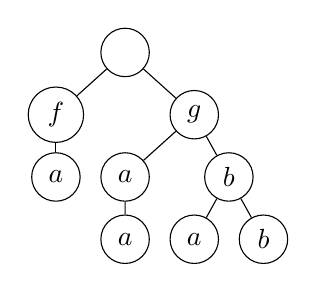
\begin{tikzpicture}[level distance=2.25em, sibling distance=5em,
%  edge from parent path={(\tikzparentnode.south) -- ++(0,-0.5em)
%   -| (\tikzchildnode.north)},
  every node/.style = {shape=circle, minimum size=1.75em, draw, align=center}]
  \node {\phantom{x}}
    child { node {$\cst{f}$}
      child { node %[fill=verylightgray]
        {$\cst{a}$} }
    }
    child { node % [fill=verylightgray]
      {$\cst{g}$}
      child { node {$\cst{a}$}
        child { node % [fill=verylightgray]
          {$\cst{a}$} }
      }
      child[sibling distance=2.5em] { node {$\cst{b}$}
        child { node %[fill=verylightgray]
          {$\cst{a}$} }
        child { node %[fill=verylightgray]
          {$\cst{b}$} }
      }
    }
    ;
\end{tikzpicture}
}}
&&
  \vcenter{\hbox{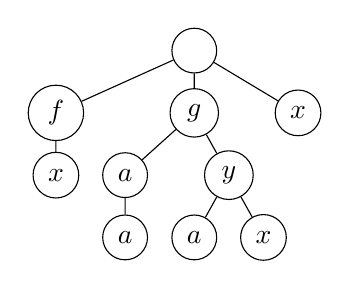
\begin{tikzpicture}[level distance=2.25em, sibling distance=5em,
%  edge from parent path={(\tikzparentnode.south) -- ++(0,-0.5em)
%   -| (\tikzchildnode.north)},
  every node/.style = {shape=circle,
    draw, align=center}]
  \node {\phantom{x}}
    child { node {$\cst{f}$}
      child { node %[fill=verylightgray]
        {$x$} }
    }
    child { node % [fill=verylightgray]
      {$\cst{g}$}
      child { node {$\cst{a}$}
        child { node % [fill=verylightgray]
          {$\cst{a}$} }
      }
      child[sibling distance=2.5em] { node {$y$}
        child { node %[fill=verylightgray]
          {$\cst{a}$} }
        child { node %[fill=verylightgray]
          {$x$} }
      }
    }
    child[sibling distance=3.75em] { node {$x$} }
    ;
\end{tikzpicture}
}}
\end{align*}
%
Assuming $\cst{a}, \cst{b}, x, y : \iota$, $\cst{f} : \iota \to \iota$,
and $\cst{g} : \iota^2 \to \iota$,
$D_1$ represents the term set
$\{
\cst{f}(\cst{a})
{,}\allowbreak\;
\cst{g}(\cst{a}, \cst{a})
{,}\allowbreak\;
\cst{g}(\cst{b}, \cst{a})
{,}\allowbreak\;
\cst{g}(\cst{b}, \cst{b})
\}$,
and $D_2$ represents the term set
$\{
\cst{f}(x)
{,}\allowbreak\;
\cst{g}(\cst{a}, \cst{a})
{,}\allowbreak\;
\cst{g}(y, \cst{a})
{,}\allowbreak\;
\cst{g}(y, x)
{,}\;
x
\}$.
%
E uses perfect discrimination trees for finding generalizations of
query terms. Thus, if the query term is
$\cst{g}(\cst{a}, \cst{a})$, it would follow the path $\cst{g}.\cst{a}.\cst{a}$
in~$D_1$ and return $\{\cst{g}(\cst{a}, \cst{a})\}.$
For~$D_2$, it would also explore paths labeled with
variables, binding them as it proceeds, and return $\{
\cst{g}(\cst{a}, \cst{a}){,}\allowbreak\; \cst{g}(y, \cst{a}){,}\allowbreak\; \cst{g}(y, x){,}\; x \}.$

It is crucial for this data structure that distinct terms always give rise to
distinct serialized terms. Conveniently, this property also holds for \lfhol{}
terms. Suppose that two distinct \lfhol{} terms yield the same serialization.
Clearly, they must disagree on parentheses; one will have the subterm $s\; t\;
u$ where the other has $s\; (t\; u).$ However, these two subterms cannot both
be well typed.

\looseness=-1
When generalizing the data structure to \lfhol, we face a complication
due to partial application. First-order terms can only be stored in leaf nodes,
but in Ehoh we must also be able to represent partially applied terms,
such as $\cst{f}$, $\cst{g}$, or $\cst{g}\;\cst{a}$ (assuming, as above, that
$\cst{f}$ is unary and $\cst{g}$ is binary). Conceptually, this can be solved
by storing a Boolean on each node indicating whether it is an accepting state.
In the implementation, the change is more subtle, because several parts of E's
code implicitly assume that only leaf nodes are accepting.

\newcommand\TermStack{\ensuremath{T}}
\newcommand\BTStack{\ensuremath{P}}

The main difficulty specific to \lfhol{} concerns applied variables. To
enumerate all generalizing terms, E needs to backtrack from child to
parent nodes. This is achieved using two stacks that store subterms of
the query term:
\TermStack{} %(\texttt{term\_\allowbreak stack})
stores the terms that
must be matched in turn against the
current subtree, and
\BTStack{} %(\texttt{term\_\allowbreak proc})
stores, for each node from
the root to the current subtree, the corresponding processed term.

Let $[a_1, \dots, a_n]$ denote an $n$-item stack with $a_1$ on top. Given a
query term $t$, the matching procedure starts at the root with $\sigma =
\emptyset$, $\TermStack{} = [t]$, and $\BTStack = []$.
%
The procedure advances by repeatedly moving to a suitable child node:
%
\begin{enumerate}
\item[A.] If the node is labeled with a symbol $\cst{f}$ and the top item
  $t$ of \TermStack{} is \confrep{}{of the form }$\cst{f}(\tuple{t}{n})$,
  replace $t$ by $n$~new items $t_1,\dots,t_n$, and push $t$ onto \BTStack.

\smallskip
\item[B.] If the node is labeled with a variable $x$, there are two subcases.
  If $x$ is already bound, check that $\sigma(x) = t$;
  otherwise, extend $\sigma$ so that $\sigma(x) = t.$ Next, pop the term $t$
  from \TermStack{} and push it onto \BTStack.
\end{enumerate}

%
The goal is to reach an accepting node. If the query term and all the terms
stored in the tree are first-order, \TermStack{} will then be empty, and the
entire query term will have been matched.
%
Backtracking works in reverse: Pop a term $t$ from \BTStack; if the current
node is labeled with an $n$-ary symbol, discard \TermStack{}'s topmost
$n$~items; push $t$ onto \TermStack. Undo any variable bindings.

As an example, looking up $\cst{g}(\cst{b}, \cst{a})$ in the tree $D_1$
would result in the following succession of stack states, starting from the
root $\varepsilon$ along the path $\cst{g}.\cst{b}.\cst{a}$:
%
\[\begin{array}{@{}l@{\kern1.5em}l@{\kern1em}l@{\kern1em}l@{\kern1em}l@{}}
& \varepsilon & \cst{g} & \cst{g}.\cst{b} & \cst{g}.\cst{b}.\cst{a} \\[.5\jot]
\sigma{:} & \emptyset & \emptyset & \emptyset & \emptyset \\
\TermStack{:} & [\cst{g}(\cst{b}, \cst{a})] & [\cst{b}, \cst{a}] & [\cst{a}] & [\,] \\
\BTStack{:} & [\,] & [\cst{g}(\cst{b}{,}\; \cst{a})] & [\cst{b}{,}\; \cst{g}(\cst{b}{,}\; \cst{a})] & [\cst{a}{,}\; \cst{b}{,}\; \cst{g}(\cst{b}, \cst{a})]
\end{array}\]
%
Backtracking amounts to moving leftward:
To get back from $\cst{g}$ to the root, we pop $\cst{g}(\cst{b}, \cst{a})$
from \BTStack, we discard two items from \TermStack{}, and we push
$\cst{g}(\cst{b}, \cst{a})$ onto \TermStack{}.

To adapt the procedure to \lfhol{}, the key idea is that an applied variable
is not very different from an applied symbol. A node labeled with an $n$-ary
head~$\zeta$ matches a prefix~$t'$ of the $k$-ary term $t$
popped from \TermStack{} and leaves $n - k$ arguments $\overline{u}$ to be
pushed back, with $t = t' \; \overline{u}.$ If $\zeta$ is a variable, it must
be bound to the prefix~$t'$ assuming $\zeta$ and $t'$ are of same type.
%
Backtracking works analogously: Given the arity $n$ of the node label $\zeta$
and the arity $k$ of the term $t$ popped from \BTStack{}, we discard the
topmost $n - k$ items $\overline{u}$ from \BTStack.

\looseness=-1
To illustrate the procedure, we consider the tree $D_2$ but change $y$'s type
to $\iota \to \iota.$ This tree stores
$\{
\cst{f}\; x
{,}\allowbreak\;
\cst{g}\; \cst{a}\; \cst{a}
{,}\allowbreak\;
\cst{g}\; (y\; \cst{a})
{,}\allowbreak\;
\cst{g}\; (y\; x)
{,}\allowbreak\;
x
\}.$
Let $\cst{g}\; (\cst{g}\;\cst{a}\;\cst{b})$ be the query term.
We have the following sequence of substitutions $\sigma$ and stacks
$\TermStack, \BTStack$:
%
\[\begin{array}{@{}l@{\kern1em}l@{\kern1em}l@{\kern1em}l@{}}
\varepsilon & \cst{g} & \cst{g}.y & \cst{g}.y.x \\[.5\jot]
\emptyset & \emptyset & \{y \mapsto \cst{g}\> \cst{a}\} & \{y \mapsto \cst{g}\> \cst{a}{,}\; x \mapsto \cst{b}\} \\[0pt]
[\cst{g}\> (\cst{g}\> \cst{a}\> \cst{b})] & [\cst{g}\> \cst{a}\> \cst{b}] & [\cst{b}] & [\,] \\[0pt]
[\,] & [\cst{g}\> (\cst{g}\> \cst{a}\> \cst{b})] & [\cst{g}\> \cst{a}\> \cst{b}{,}\;\cst{g}\> (\cst{g}\> \cst{a}\> \cst{b})] & [\cst{b}{,}\;\cst{g}\> \cst{a}\> \cst{b}{,}\;\cst{g}\> (\cst{g}\> \cst{a}\> \cst{b})]
\end{array}\]

\confrep{}{When backtracking from $\cst{g}.y$ to $\cst{g}$, by comparing
$y$'s arity of $n = 1$ with $\cst{g}\; \cst{a}\; \cst{b}$'s arity of $k = 0$,
we determine that one~item must be discarded from \TermStack{}. }%
Finally, to avoid traversing twice as many subterms as in the first-order
case, we can optimize prefixes: Given a
query term $\zeta\;\tuple{t}{n}$, we can also match prefixes
$\zeta\;\tuple{t}{k}$, where $k < n$, by allowing \TermStack{} to be nonempty when we reach an accepting node.
%If accepting nodes correspond to legal prefixes, the stack will then contain
%exactly the remaining arguments: $[t_{k+1},\dots,t_n].$

\newcommand\quadruple{\mathcalx{Q}}
Similarly to unification and matching, we present finding generalizations
in a perfect discrimination tree as a transition system. States
are quadruples $\quadruple = (\overline{t}, \overline{b}, \mathit{D}, \sigma)$, where
$\overline{t}$ is a list of terms, $\overline{b}$ is a list of tuples storing
backtracking information, $\mathit{D}$ is a discrimination
(sub)tree, and $\sigma$ is a substitution.

%With $+$ we denote list append operation, and with
%$::$ we denote operation of prepending single element to list.

Let $D$ be a perfect discrimination tree. $\Term(D)$ denotes the set of terms
stored in $D$. The function $D|_\zeta$ returns the child of $D$ labeled with
$\zeta$, if it exists. Child nodes are themselves perfect discrimination
(sub)trees. Given any node $D$, if the node is accepting, then the value stored
on that node is defined as $\mathit{val}(D) = (s, d)$, where $s$ is the
accepted term and $d$ is some arbitrary data;
%(typically, an equation whose one side is~$s$)
otherwise, $\mathit{val}(D)$ is undefined.

%We label the tree nodes using BFS, starting with 0 as label for
%root node.

%With $\mathcalx{R}$ we denote $(\overline{t}, \overline{b}, D, \sigma)$ or
%$(\mathit{v}, \sigma)$ or $\bot$.

Starting from an initial state $([t], [\,], D, \emptyset)$, where $t$ is the query
term and $D$ is an entire discrimination tree, the following transitions are
possible:
% \begin{description}[labelwidth=\widthof{\rm\textsf{AdvanceX}}]
%   \item[\rm\textsf{AdvanceF}]
%     $ ( \cst{f} \> \tuple{s}{m} \mathrel{\cdot} \overline{t}{,}\; \overline{b}{,}\; D{,}\; \sigma )
%         \Pdtarrow
%         (\tuple{s}{m} \cdot \overline{t}{,}\;
%         (\cst{f} \> \tuple{s}{m}, D, \sigma) \cdot \overline{b}{,}\; D{|}_\cst{f}{,}\; \sigma)
%       $\quad
%       if $D{|}_\cst{f}$ is defined
  
%   \smallskip
%   \item[\rm\textsf{AdvanceX}]
%     $ ( s \; \tuple{s}{m} \mathrel{\cdot} \overline{t}{,}\; \overline{b}{,}\; D{,}\; \sigma )
%         \Pdtarrow {}$ \\
%     $(\tuple{s}{m} \cdot \overline{t}{,}\; (s \; \tuple{s}{m}, D, \sigma) \cdot \overline{b}{,}\; D{|}_x{,}\; \sigma[x \mapsto s])
%       $\\
%       if $D{|}_x$ is defined, $x$ and $s$ have the same type, and
%       $\sigma(x)$ is either undefined or equal to $s$
  
%   \smallskip
%   \item[\rm\textsf{Backtrack}]
%     $ ( \tuple{s}{m} \cdot \overline{t}{,}\; (s, D_0, \sigma_0) \cdot \overline{b}{,}\; D{,}\; \sigma)
%         \Pdtarrow %\\\hphantom{\rm\textsf{AdvanceX}}%
%       (s \mathrel{\cdot} \overline{t}{,}\; \overline{b}{,}\; D_0{,}\; \sigma_0)$ \\
%       if $D_0{|}_\zeta = D$ and $m = \textit{arity}(\zeta) - \textit{arity}(s)$
  
%   \smallskip
%   \item[\rm\textsf{Success}]
%     $ ( [\,]{,}\; \overline{b}{,}\; D{,}\; \sigma )
%         \Pdtarrow (\mathit{val}(D){,}\; \sigma)$ \\
%     if~$\mathit{val}(D)$ is defined
% \end{description}

\noindent
\begin{tabular}{ll}
  \textsf{AdvanceF} & $ ( \cst{f} \> \tuple{s}{m} \mathrel{\cdot} \overline{t}{,}\; \overline{b}{,}\; D{,}\; \sigma )
           \Pdtarrow
           (\tuple{s}{m} \cdot \overline{t}{,}\;
           (\cst{f} \> \tuple{s}{m}, D, \sigma) \cdot \overline{b}{,}\; D{|}_\cst{f}{,}\; \sigma)
         $ \\
                   & if $D{|}_\cst{f}$ is defined \\[\jot]
  \textsf{AdvanceX} & $( s \; \tuple{s}{m} \mathrel{\cdot} \overline{t}{,}\; \overline{b}{,}\; D{,}\; \sigma ) 
                      \Pdtarrow {} 
                      (\tuple{s}{m} \cdot \overline{t}{,}\; (s \; \tuple{s}{m}, D, \sigma) \cdot \overline{b}{,}\; D{|}_x{,}\; \sigma[x \mapsto s])$ \\
                    & if $D{|}_x$ is defined, $x$ and $s$ have the same type,\\ & and
                    $\sigma(x)$ is either undefined or equal to $s$ \\[\jot]
  \textsf{Backtrack} & $ ( \tuple{s}{m} \cdot \overline{t}{,}\; (s, D_0, \sigma_0) \cdot \overline{b}{,}\; D{,}\; \sigma)
                      \Pdtarrow
                      (s \mathrel{\cdot} \overline{t}{,}\; \overline{b}{,}\; D_0{,}\; \sigma_0)$  \\
                      & if $D_0{|}_\zeta = D$ and $m = \textit{arity}(\zeta) - \textit{arity}(s)$ \\[\jot]
  \textsf{Success}    & $ ( [\,]{,}\; \overline{b}{,}\; D{,}\; \sigma ) \Pdtarrow (\mathit{val}(D){,}\; \sigma)$ \\
                      & if~$\mathit{val}(D)$ is defined
\end{tabular}

Above, $\cdot$ denotes prepending an element or a list to a list.
%
Intuitively, \textsf{AdvanceF} and \textsf{AdvanceX} move deeper in
the tree, generalizing cases A and B above to \lfhol{} terms.
\textsf{Backtrack} can be used to return to a previous state.
\textsf{Success} extracts the term~$t$ and data~$d$ stored in
an accepting node.

\newcommand\BDTARROW[1]{\rlap{\ensuremath{\Pdtarrow_{#1}\;}}\phantom{\Pdtarrow_\textsf{AdvanceX}\;}}

The following derivation illustrates how to locate a generalization of
$\cst{g}\; (\cst{g}\;\cst{a}\;\cst{b})$ in the tree $D_2$:\pagebreak[2]
%
\begin{align*}
 & ([\cst{g} \; (\cst{g} \; \cst{a} \; \cst{b})]{,}\;  [\,]{,}\;  D{,}\;  \emptyset) \\[-1\jot]
 \BDTARROW{\textsf{AdvanceF}}&
 ([\cst{g} \; \cst{a} \; \cst{b}]{,}\;  [(\cst{g} \; (\cst{g} \; \cst{a} \; \cst{b}), D, \emptyset)]{,}\;  D{|}_{\cst{g}}{,}\;  \emptyset)\\[-1\jot]
 \BDTARROW{\textsf{AdvanceX}}&
 ([\cst{b}]{,}\;  [(\cst{g} \; \cst{a} \; \cst{b}, D{|}_{\cst{g}}, \emptyset), \ldots]{,}\;  D{|}_{\cst{g}.y}{,}\;  \{y \mapsto \cst{g} \; \cst{a} \}) \\[-1\jot]
 \BDTARROW{\textsf{AdvanceX}}&
 ([\,]{,}\;  [(\cst{b}, D{|}_{\cst{g}.y}, \{y \mapsto \cst{g} \; \cst{a} \}), \ldots]{,}\; D{|}_{\cst{g}.y.x}{,}\; \{ y \mapsto \cst{g} \; \cst{a}{,}\; x \mapsto \cst{b} \}) \\[-1\jot]
 \BDTARROW{\textsf{Success}}& ((\cst{g} \; (y \; x), d){,}\; \{ y \mapsto \cst{g} \; \cst{a}{,}\; x \mapsto \cst{b} \})
\end{align*}

Let ${\Pdtarrow_{\mathsf{Advance}}} = {\Pdtarrow_{\mathsf{AdvanceF}}} \cup
{\Pdtarrow_{\mathsf{AdvanceX}}}$.
%and ${\Pdtarrow_{\mathsf{NoBacktrack}}} = {\Pdtarrow_{\mathsf{Advance}}} \cup
%{\Pdtarrow_{\mathsf{Success}}}$.
It is easy to show that \textsf{Backtrack} undoes an \textsf{Advance}
transition: % and can be avoided when starting from an initial state.

\begin{lemma}\label{lemma:ehoh:backtrack-inverses-advance} If $\quadruple \Pdtarrow_{\mathsf{Advance}} \quadruple'$, then
  $\quadruple' \Pdtarrow_{\mathsf{Backtrack}} \quadruple$.
  \end{lemma}
\begin{proof}
For both \textsf{Advance} steps, we show that \textsf{Backtrack} restores the state
properly. If \textsf{AdvanceF} was applied, we have
%
\begin{align*}
  ( \cst{f} \> \tuple{s}{m} \mathrel{\cdot} \overline{t}{,}\; \overline{b}{,}\; D{,}\; \sigma )
& \Pdtarrow_{\mathsf{AdvanceF}}
  (\tuple{s}{m} \cdot \overline{t}{,}\;
      (\cst{f} \> \tuple{s}{m}, D, \sigma) \cdot \overline{b}{,}\; D{|}_\cst{f}{,}\; \sigma)
\\[-\jot]
& \Pdtarrow_{\mathsf{Backtrack}}
  ( \overline{t'}{,}\; \overline{b}{,}\; D{,}\; \sigma )
\end{align*}
We must show that $\overline{t'} = \cst{f} \> \tuple{s}{m} \mathrel{\cdot} \overline{t}$.
Let $k = \textit{arity}(\cst{f})$ and $l = \textit{arity}(\cst{f} \> \tuple{s}{m})$.
By definition of $k$, we have $m = k - l$, as in \textsf{Backtrack}'s side
condition. Thus, $\overline{t'} = \cst{f} \> \tuple{s}{m} \mathrel{\cdot}
\overline{t}$. The other case is
\begin{align*}
  ( s \; \tuple{s}{m} \mathrel{\cdot} \overline{t}{,}\; \overline{b}{,}\; D{,}\; \sigma )
& \Pdtarrow_{\mathsf{AdvanceX}}
  (\tuple{s}{m} \cdot \overline{t}{,}\; (s \; \tuple{s}{m}, D, \sigma) \cdot \overline{b}{,}\; D{|}_x{,}\; \sigma')
\\[-\jot]
& \Pdtarrow_{\mathsf{Backtrack}}
  ( \overline{t'}{,}\; \overline{b}{,}\; D{,}\; \sigma )
\end{align*}
where $\sigma' = \sigma[x \mapsto s]$.
Again, we must show that $\overline{t'} = s \; \tuple{s}{m} \mathrel{\cdot} \overline{t}$. Terms
$x$ and $s$ must have the same type for \textsf{AdvanceX} to be applicable; therefore, they have the same arity. Then, we conclude $m=
\textit{arity}(s) - \textit{arity}(s \; \tuple{s}{m} ) =  \textit{arity}(x) - \textit{arity}(s \; \tuple{s}{m} )$, as in \textsf{Backtrack}'s
side condition. Thus, $\overline{t'} = s \; \tuple{s}{m} \mathrel{\cdot} \overline{t}$.
\end{proof}

\begin{lemma}\label{lemma:ehoh:advance-inverses-backtrack}
  If $\quadruple \Pdtarrow_{\mathsf{Advance}} \quadruple'
  \Pdtarrow_{\mathsf{Backtrack}} \quadruple''$, then
  $\quadruple'' = \quadruple$.
  \end{lemma}
\begin{proof}
  By Lemma~\ref{lemma:ehoh:backtrack-inverses-advance}, $\quadruple'
  \Pdtarrow_{\mathsf{Backtrack}} \quadruple$. Furthermore, \textsf{Backtrack} is
  clearly functional. Thus, $\quadruple'' = \quadruple$.
\end{proof}

\begin{lemma}\label{lemma:ehoh:backtrack-remove}
  Let $\quadruple = ([t], [\,], D, \emptyset)$. If $\quadruple
  \Pdtarrow^* \quadruple'$, then $\quadruple \Pdtarrow_{\mathsf{Advance}}^*\allowbreak
  \quadruple'$.
\end{lemma}
  
\begin{proof}
  \looseness=-1
  Let $\quadruple = \quadruple{}_{\,\,0} \Pdtarrow \cdots \Pdtarrow \quadruple{}_{\,\,n} = \quadruple'$.
  Let $i$ be the index of the first transition of the form $\quadruple{}_{\,\,i} \Pdtarrow_{\mathsf{Backtrack}}
  \quadruple{}_{\,\,i+1}$. Since $\quadruple{}_{\,\,0}$'s backtracking stack is empty, we must
  have $i \not= 0$. Hence, we have $\quadruple{}_{\,\,i-1} \Pdtarrow_{\mathsf{Advance}}
  \quadruple{}_{\,\,i} \Pdtarrow_{\mathsf{Backtrack}} \quadruple{}_{\,\,i+1}$. By
  Lemma~\ref{lemma:ehoh:advance-inverses-backtrack}, $\quadruple{}_{\,\,i-1} =
  \quadruple{}_{\,\,i+1}$. Thus, we can shorten the derivation to $\quadruple{}_{\,\,0}
  \Pdtarrow \cdots \Pdtarrow \quadruple{}_{\,\,i-1} = \quadruple{}_{\,\,i+1} \Pdtarrow
  \cdots \Pdtarrow \quadruple{}_{\,\,n}$,
  thereby eliminating one \textsf{Backtrack} transition. By repeating this
  process, we eliminate all \textsf{Backtrack} transitions.
\end{proof}

\begin{lemma}\label{lemma:ehoh:termination-pdt}
  There exist no infinite chains of the form
  $\quadruple{}_{\,\,0} \Pdtarrow_\mathsf{Advance}\allowbreak \quadruple{}_{\,\,1} \Pdtarrow_\mathsf{Advance}
  \cdots$.
\end{lemma}
\begin{proof}
  With each \textsf{Advance} transition, the height of the discrimination tree
  decreases by at least one.
\end{proof}


Perfect discrimination trees match a single term against a set of terms. To
prove them correct, we will connect them to the transition system
$\Matcharrow$ for matching (Sect.~\ref{sec:ehoh:unif-match}). This connection\pagebreak[2] will
help us show that whenever a discrimination tree stores a generalization of a
query term, this generalization can be found.
%
To express the refinement, we introduce an intermediate transition
system, $\Matchiiarrow$, that focuses on a single pair of terms (like
$\Matcharrow$) but that solves the constraints in a depth-first, left-to-right
fashion and builds the substitution incrementally (like $\Pdtarrow$).
Its initial states are of the form $([s \MATCH t], \emptyset)$. Its transitions
are as follows:

\vskip\abovedisplayskip
\noindent
\begin{tabular}{ll}
  \textsf{Decompose} & $ (\cst{f} \; \tuple{s}{m} \MATCH \cst{f} \; \tuple{t}{m} \mathrel{\cdot} \overline{c}, \, \sigma) \Matchiiarrow {} ( (s_1 \MATCH t_1, \ldots, s_m \MATCH t_m) \cdot \overline{c}, \sigma ) $ \\[\jot]
  \textsf{DecomposeX} & $(x \; \tuple{s}{{m}} \MATCH u \; \tuple{t}{{m}} \mathrel{\cdot} \overline{c}, \, \sigma) \Matchiiarrow {} ( (s_1 \MATCH t_1, \ldots, s_m \MATCH t_m) \cdot \overline{c}, \sigma[x \mapsto u] )$ \\
                    & if $x$ and $u$ have the same type and either $\sigma(x)$ is undefined or $\sigma(x)=u$ \\[\jot]
  \textsf{Success} & $ ([\,], \, \sigma) \Matchiiarrow  \sigma $ \\[\jot]
  \textsf{Clash}    & $ (\cst{f} \; \tuple{s}{m} \MATCH \cst{g} \; \tuple{t}{n} \mathrel{\cdot} \overline{c}, \, \sigma) \Matchiiarrow \bot $ \\[\jot]
  \textsf{ClashTypeX}    & $(x \; \tuple{s}{{m}} \MATCH u \; \tuple{t}{{m}} \mathrel{\cdot} \overline{c}, \, \sigma) \Matchiiarrow \bot$ \\
                         & if~$x$ and $u$ have different types  \\[\jot]
  \textsf{ClashLenXF}    & $(x \; \tuple{s}{{m}} \MATCH \cst{f} \; \tuple{t}{{n}} \mathrel{\cdot} \overline{c}, \, \sigma) \Matchiiarrow \bot$ \\
                         & if~$m > n$  \\[\jot]
  \textsf{ClashLenXY}    & $(x \; \tuple{s}{{m}} \MATCH y \; \tuple{t}{{n}} \mathrel{\cdot} \overline{c}, \, \sigma) \Matchiiarrow \bot$ \\
                         & if~$x \neq y$ and $m > n$ \\[\jot]
  \textsf{ClashFX}    & $(\cst{f} \; \overline{s} \MATCH x \; \overline{t}  \mathrel{\cdot} \overline{c}, \, \sigma) \Matchiiarrow \bot$ \\[\jot]
  \textsf{Double}    & $(x \; \tuple{s}{{m}} \MATCH u \; \tuple{t}{{m}}  \mathrel{\cdot} \overline{c}, \, \sigma) \Matchiiarrow \bot$ \\
                     & if $x$ and $u$ have the same type, $\sigma(x)$ is defined, and $\sigma(x) \neq u$ \\[\jot]
\end{tabular}
\vskip\belowdisplayskip
\newcommand\AlphaMatch[1]{\alpha(#1)}
We need an auxiliary function to convert $\Matchiiarrow$ states to
$\Matcharrow$ states.
Let
$\AlphaMatch{\{ x_1 \mapsto s_1,\allowbreak \ldots, x_m \mapsto s_m \}}
 = \{ x_1 \MATCH s_1,\ldots,\,\allowbreak x_m \MATCH s_m \}$,
$\AlphaMatch{\overline{c}, \sigma} =
\{ c \mid c \in \overline{c} \} \mathrel\cup \AlphaMatch{\sigma}$, and
$\AlphaMatch{\bot} = \bot$.
%
Moreover, let $\mathcal{S}$ range over states of the form $(\overline{c}, \sigma)$ and
$\mathcalx{R}$ additionally range over special states of the form $\sigma$ or
$\bot$.


\begin{lemma}\label{lemma:ehoh:match-refinement}
  If $\mathcal{S} \Matchiiarrow \mathcalx{R}$,
  then $\AlphaMatch{\mathcal{S}} \Matcharrow^* \AlphaMatch{\mathcalx{R}}$.
\end{lemma}
\begin{proof}
By case distinction on $\mathcalx{R}$. Let $\mathcal{S} = (\overline{c}, \sigma)$.

\medskip

\begin{sloppypar}%
  \noindent
  \textsc{Case} $\mathcalx{R} = (\overline{c'}, \sigma')$:\enskip
  Only $\Matchiiarrow_{\mathsf{Decompose}}$ and
  $\Matchiiarrow_{\mathsf{DecomposeX}}$ are possible.
  If $\Matchiiarrow_{\mathsf{Decompose}}$ is applied, then $\Matcharrow_{\mathsf{Decompose}}$
  is applicable and results in $\AlphaMatch{\mathcalx{R}}$.
  If $\Matchiiarrow_{\mathsf{DecomposeX}}$ is applied,
  we have either $m>0$, and $\Matcharrow_{\mathsf{DecomposeX}}$ is applicable,
  or $m = 0$, and $\AlphaMatch{\overline{c'},\sigma'} = \AlphaMatch{\mathcal{S}}$,
  which implies that the two states are connected by an idle transition of
  $\Matcharrow^*$.
  \end{sloppypar}
  
  \medskip
  
  \noindent
  \textsc{Case} $\mathcalx{R} = \bot$:\enskip
  All the $\Matchiiarrow$ rules resulting in $\bot$ except for \textsf{Double}
  have the same side conditions as the corresponding $\Matcharrow$ rules.
  $\Matchiiarrow_{\mathsf{Double}}$ corresponds to
  $\Matcharrow_{\mathsf{Double}}$ if $m=0$. If $m \neq 0$, we need
  an intermediate $\Matcharrow_{\mathsf{DecomposeX}}$ step before
  $\Matcharrow_{\mathsf{Double}}$ can be applied to derive $\bot$. Since
  $\Matchiiarrow_{\mathsf{Double}}$ is applicable, $\sigma(x) = u'
  \neq u$. Hence, $x \MATCH u'$ must be present in $\AlphaMatch{\overline{c},
  \sigma}$. $\Matcharrow_{\mathsf{DecomposeX}}$ will augment this set with
  $x \MATCH u$, enabling $\Matcharrow_{\mathsf{Double}}$.
  
  \medskip
  
  \noindent
  \textsc{Case} $\mathcalx{R} = \sigma$:\enskip
  The only possible rule is $\Matchiiarrow_{\mathsf{Success}}$,
  with $\overline{c}=[\,]$. Since $\AlphaMatch{\mathcal{S}} = \AlphaMatch{\sigma}$,
  this transition corresponds to an idle transition of $\Matcharrow^*$.
\end{proof}

\begin{lemma}\label{lemma:ehoh:refined-match-partial-correctness}\,%
  If $\mathcal{S} \Matchiiarrow^{!} \mathcalx{R}$, then $\mathcalx{R}$ is either
  some substitution $\sigma'$ or $\bot$.
  If $\mathcal{S} \Matchiiarrow^{!} \sigma'$, then $\sigma'$ is the MGG
  of~$\AlphaMatch{\mathcal{S}}$.
  If $\mathcal{S} \Matchiiarrow^{!} \bot$, then $\AlphaMatch{\mathcal{S}}$ has
  no solutions.
  \end{lemma}
\begin{proof}
  %Let $\mathcal{S} = (\overline{c}, \sigma)$.
  
  First, we show that states $\mathcal{S}' = (\overline{c'}, \sigma')$ cannot be
  normal forms, by exhibiting transitions from such states. If $\overline{c'} =
  [\,]$, the $\Matchiiarrow_{\mathsf{Success}}$ rule would apply. Otherwise, let
  $\overline{c'} = c_1 \cdot \overline{c''}$ and consider the matching problem
  $\{c_1\} \cup \AlphaMatch{\sigma'}$. If this problem is in solved form, $c_1$
  is a constraint corresponding to a solved variable, and we can apply
  $\Matchiiarrow_{\mathsf{DecomposeX}}$ to move the constraint into the
  substitution. Otherwise, some $\Matcharrow$ rule can be applied. It
  necessarily focuses on $c_1$, since the constraints from
  $\AlphaMatch{\sigma'}$ correspond to solved variables. In all cases except for
  $\Matcharrow_{\mathsf{DecomposeX}}$, a homologous
  $\Matchiiarrow$ rule  can be applied to $\mathcal{S}'$. If $\Matcharrow_{\mathsf{DecomposeX}}$
  would make $\Matcharrow_{\mathsf{Double}}$ applicable, then we can apply $\Matchiiarrow_{\mathsf{Double}}$ to $\mathcal{S}'$;
  otherwise, $\Matchiiarrow_{\mathsf{DecomposeX}}$ is applicable.
  
  Second, by Lemma \ref{lemma:ehoh:match-refinement},
  if $\mathcal{S} \Matchiiarrow^{!} \sigma'$, then
  $\AlphaMatch{\mathcal{S}} \Matcharrow^* \AlphaMatch{\sigma'}$.
  By construction, $\AlphaMatch{\sigma'}$ is in solved form.
  Therefore, $\AlphaMatch{\mathcal{S}} \Matcharrow^{!} \AlphaMatch{\sigma'}$.
  By completeness of $\Matcharrow$, the substitution corresponding to
  $\AlphaMatch{\sigma'}$---that is, $\sigma'$---is the MGG of~$\AlphaMatch{\mathcal{S}}$.
  
  Third, by Lemma~\ref{lemma:ehoh:match-refinement}, if $\mathcal{S}
  \Matchiiarrow^{!} \bot$, then $\AlphaMatch{\mathcal{S}} \Matcharrow^{!} \bot$.
  By soundness of $\Matcharrow$, $\AlphaMatch{\mathcal{S}}$ has
  no solutions.
\end{proof}


\begin{lemma}\label{lemma:ehoh:refined-match-termination}\,%
  The relation $\Matchiiarrow$ is well founded.
  \end{lemma}
\begin{proof}
  By Lemma \ref{lemma:ehoh:match-refinement}, every $\Matchiiarrow$ transition
  corresponds to zero or more $\Matcharrow$ transitions.
  Since $\Matcharrow$ is well founded,
  the only transitions that can violate well-foundedness of $\Matchiiarrow$ are
  the ones that take idle $\Matcharrow^*$ transitions:
  $\Matchiiarrow_{\mathsf{DecomposeX}}$ for $m=0$ and
  $\Matchiiarrow_{\mathsf{Success}}$. The latter is terminal, so it cannot
  contribute to infinite chains.
  As for $\Matchiiarrow_{\mathsf{DecomposeX}}$, with $m=0$,
  it decreases the following measure~$\mu$, which the other rules nonstrictly
  decrease, with respect to the multiset extension of $<$ on natural numbers:
  $\mu([s_1 \MATCH t_1, \ldots, s_m \MATCH t_m], \sigma) =
    \{\left|s_1\right|, \ldots \left|s_m\right|\}$,
  where $\left|s\right|$ denotes the syntactic size of $s$.
\end{proof}
  
\begin{lemma}\label{lemma:ehoh:refined-matching-solution}
  If term $s$ generalizes $t$, then $([s \MATCH t], \emptyset) \Matchiiarrow^! \sigma$,
  where $\sigma$ is the MGG of $s \MATCH t$.
\end{lemma}
\begin{proof}
By Lemma \ref{lemma:ehoh:refined-match-termination}, there exists a normal form
$\mathcalx{R}$ starting from $\mathcal{S} = ([s \MATCH t],\allowbreak \emptyset)$. Since $s
\MATCH t$ is solvable, by Lemma~\ref{lemma:ehoh:refined-match-partial-correctness},
and soundness of $\Matchiiarrow$ (a consequence of Lemma \ref{lemma:ehoh:match-refinement}
and soundness of $\Matcharrow$),
$\mathcalx{R}$ must be the MGG for $s$ and~$t$.
\end{proof}


\begin{lemma}\label{lemma:ehoh:pdt-complete-help}
  If there exists a term $s \in \Term(D)$ that generalizes the query term~$t$,
  then there exists a derivation $([t], [\,],\allowbreak D,\allowbreak \emptyset) \Pdtarrow^! ((s, d),
  \sigma)$. %, where $\sigma$ is the MGG for $s$ and $t$.
  \end{lemma}
  \begin{proof}
    By Lemma \ref{lemma:ehoh:refined-matching-solution}, we know that $(s \MATCH t,
    \emptyset) \Matchiiarrow^! \sigma$ for each $s \in \Term(D)$ generalizing $t$.
    This means that there exists a derivation
    $([s \MATCH t], \emptyset) = (\overline{c_0}, \sigma_0) \Matchiiarrow \cdots \Matchiiarrow (\overline{c_n}, \sigma_n)\allowbreak \Matchiiarrow \sigma$.
    The $n$ first transitions must be \textsf{Decompose} or \textsf{DecomposeX},
    and the last transition must be \textsf{Success}.

    We show that there exists a derivation of the form
    $([t], [\,],\allowbreak D, \emptyset) = \quadruple{}_{\,\,0}\allowbreak \Pdtarrow \cdots
    \Pdtarrow \quadruple{}_{\,\,n} \Pdtarrow ((s, d),\sigma)$, where $\quadruple{}_{\,\,i} =
    (\overline{t_i}, \overline{b_i}, \allowbreak D_i, \sigma_i)$ for each $i$.
  %
    We define $\overline{t_i}$, $\overline{b_i}$, and $D_i$ as follows, for $i > 0$.
    The list $\overline{t_i}$ consists of the right-hand sides of the
    constraints~$\overline{c_i}$, in the same order.
    %todo:
    Let $\mathit{hd}$ be the function that extracts the head of a list. We set
          $b_i = (\mathit{hd}(\overline{t_{i-1}}),\allowbreak D_{i-1}, \sigma_{i-1})$. We know that $\overline{c_{i-1}}$ is
          nonempty, since there exists a transition $(\overline{c_{i-1}}, \sigma_{i-1}) \Matchiiarrow (\overline{c_i}, \sigma_i)$%
          ; thus, $\overline{t_{i-1}}$ is nonempty.
    If an accepting node storing~$s$ was reached in $n$~steps, the
      serialization of $s$ must be of the form $\zeta_1.\cdots.\zeta_n$. Take $D_i
      = D_{i-1}{|}_{\zeta_i}$.
  
    The sequence of states $\quadruple{}_{\,\,i}$ forms a
    derivation:
    If $(\overline{c_i},\allowbreak \sigma_i)\allowbreak \Matchiiarrow_\textsf{Decompose}
    (\tuple{c}{{i+1}},\allowbreak \sigma_{i+1})$, then $\quadruple{}_{\,\,i}
    \Pdtarrow_\textsf{AdvanceF} \allowbreak \quadruple{}_{\,\,i+1}$.
    If $(\overline{c_i},\allowbreak \sigma_i) \Matchiiarrow_\textsf{DecomposeX}
    (\tuple{c}{{i+1}},\allowbreak \sigma_{i+1})$, then $\quadruple{}_{\,\,i}
    \Pdtarrow_\textsf{AdvanceX} \quadruple{}_{\,\,i+1}$.
    If $(\overline{c_n},\allowbreak \sigma_n) \Matchiiarrow_\textsf{Success} \sigma$, then
    $\quadruple{}_{\,\,n} \Pdtarrow_\textsf{Success} ((s, d),\allowbreak \sigma)$.
\end{proof}
  
\begin{lemma}\label{lemma:ehoh:pdt-soundi}
  If $([t], [\,], D, \emptyset) \Pdtarrow^+ ((s, d), \sigma)$, then $s \in \Term(D)$
  and $\sigma$ is the MGG of $s \MATCH t$.
  \end{lemma}
  
  \begin{proof}
  Let $([t], [\,], D, \emptyset) =
  \quadruple{}_{\,\,0} \Pdtarrow \cdots \Pdtarrow \quadruple{}_{\,\,n}
  \Pdtarrow ((s, d), \sigma)$ be a derivation, where $\quadruple{}_{\,\,i} =
  (\overline{t_i}, \overline{b_i},\allowbreak D_i, \sigma_i)$ for each $i$. Without loss of
  generality, by Lemma \ref{lemma:ehoh:backtrack-remove}, we can assume that the
  derivation contains no \textsf{Backtrack} transitions.
  
  The first conjunct, $s \in \Term(D)$, clearly holds
  %by definition --- some invariant must be needed here
  for any term found
  from an initial state. To prove the second conjunct, we first introduce a
  function $\mathit{preord}$ that defines the preorder decomposition of a list
  of terms:
  $\mathit{preord}([\,]) = [\,]$ and
  $\mathit{preord}(\zeta \; \tuple{s}{n} \cdot \overline{xs}) =
  (\zeta{,}\; \tuple{s}{n} \cdot \overline{xs}) \cdot \mathit{preord}(\tuple{s}{n} \cdot \overline{xs})$.
  %
  Given a term~$s$, $\mathit{preord}([s])$ gives a sequence
  $(\zeta_1, \tuple{u}{1}), \dots, \allowbreak
  (\zeta_n, \tuple{u}{n})$.
  Since $s \in \Term(D)$,
  the sequence $D_0, \ldots, D_n$ follows the preorder serialization of $s$:
  $D_i = D_{i-1}|_{\zeta_i}$ for $i > 0$.
  
  Next, we show that there exists a derivation of the form
  $([s \MATCH t], \emptyset) = \mathcal{S}_0 \Matchiiarrow
  \cdots \Matchiiarrow \mathcal{S}_n \Matchiiarrow \sigma$, where
  $\mathcal{S}_i = (\overline{c_i}, \sigma_i)$. We define $\overline{c_i}$, for $i>0$,
  as the list of constraints whose left-hand sides are the elements of $\overline{u_i}$
  and right-hand sides are the elements of $\overline{t_i}$, in the order they appear in the respective lists.
  By inspecting the definition of $\mathit{preord}$
  and the changes each \textsf{Advance} step makes
  to the head of $\overline{t_i}$, we can see that $\overline{u_i}$ and $\overline{t_i}$  have the same length.
  The sequence of states $\mathcal{S}_i$ forms a derivation:
  %
  If $\quadruple{}_{\,\,i} \Pdtarrow_\textsf{AdvanceF} \quadruple{}_{\,\,i+1}$, then $\mathcal{S}_i \Matchiiarrow_\textsf{Decompose} \mathcal{S}_{i+1}$.
  If $\quadruple{}_{\,\,i} \Pdtarrow_\textsf{AdvanceX} \quadruple{}_{\,\,i+1}$, then $\mathcal{S}_i\allowbreak \Matchiiarrow_\textsf{DecomposeX} \mathcal{S}_{i+1}$.
  If $\quadruple{}_{\,\,n} \Pdtarrow_\textsf{Success} \sigma$, then
  $\mathcal{S}_n\allowbreak \Matchiiarrow_\textsf{Success} \sigma$.
\end{proof}
  
\begin{theorem}[Total Correctness]\label{theorem:ehoh:pdt-complete}\,%
  Let $D$ be a perfect discrimination tree and $t$ be a term.
  The sets $\{ s \in \Term(D) \mid \exists \sigma.\; \sigma(s) = t \}$
  and $\{ s \mid \exists d, \sigma.\; ([t], [\,], D, \emptyset) \allowbreak
  \Pdtarrow^! ((s, d), \sigma) \}$ are equal.
\end{theorem}
\begin{proof}
  This follows from Lemmas \ref{lemma:ehoh:pdt-complete-help} and \ref{lemma:ehoh:pdt-soundi}.
\end{proof}

The theorem tells us that given a term~$t$, all generalizations $s$ stored
in the perfect discrimination tree can be found, but it does not exclude
nondeterminism. Often, both \textsf{AdvanceF} and \textsf{AdvanceX} are
applicable. To find all generalizations, we need to follow both transitions.
But for some applications, it is enough to find a single generalization.

To cater for both types of applications, E provides iterators that store the
state of a traversal. After an iterator is initialized
with the root node $D$ and the query term $t$, each call to
\textsc{FindNextVal} will move the iterator to the next node that generalizes
the query term and stores a value, indicating an accepting node. After all
such nodes have been traversed, the iterator is set to point to
$\mathit{Null}$.

The following definitions constitute the high-level interface for
iterating through values incrementally or for obtaining all values of nodes that
store generalizations of the query term in $D$.


\begin{quotex}
  \MyFunction{InitIter}{PDTNode $D$, Term $t$}
  \q $i \gets \textsc{Iterator}()$ \\
  \q $(i.\mathit{node}, i.\mathit{t\_stack}, i.\mathit{t\_proc}, i.\mathit{c\_iter}) \gets (D, [t], [\,], \textit{Start})$ \\
  \q \MyReturn $i$
  
  \vskip 1.5\jot
  
  \MyProcedure{FindNextVal}{Iterator $i$}
  \q \MyDo
  \qq \textsc{FindNextNode}($i$) \\
  \q \MyWhileOfDo{$i.\mathit{node} \not= \mathit{Null} \mathrel\land
    \\ \qqq  (\lnot\, i.\mathit{t\_stack}.\mathit{isEmpty}()
    \mathrel\lor \lnot\, i.\mathit{node}.\mathit{has\_val}())$}
  
  \vskip 1.5\jot
  
  \MyFunction{AllVals}{PDTNode $D$, Term $t$}
  \q $\mathit{i} \gets \textsc{InitIter}(D, t)$ \\
  \q $\textsc{FindNextVal}(i)$ \\
  \q $\mathit{res} \gets \emptyset$ \\
  \q \MyWhile{$\mathit{i.node} \neq \mathit{Null}$}
  \qq $\mathit{res} \gets \mathit{res} \cup \{ \mathit{i.node.val()} \}$ \\
  \qq $\textsc{FindNextVal}(i)$
  \\[\jot]
  \q \MyReturn $\mathit{res}$
  \end{quotex}
  
  The core functionality is implemented in \textsc{FindNext\-Node}, presented below. This
  procedure moves the iterator to the next node that has not been explored in the
  search for generalization, or \textit{Null} if the entire tree has been
  traversed. It first goes through all child nodes labeled with a variable before
  possibly visiting the child node labeled with a function symbol. We assume that
  we can iterate through the children of a node using a function
  \textsc{NextVarChild} that, given a tree node and iterator through children,
  advances the iterator to the child representing the next variable. Furthermore, we
  assume that the iterator can also be in the distinguished states \textit{Start}
  and \textit{End}.
  \textit{Start} indicates that no child has been visited yet; \textit{End}
  indicates that we have visited all children. Finally, the expression
  $n.\mathit{child}(\zeta)$ returns a child of the node $n$ labeled $\zeta$ if
  such a child exists or $\mathit{Null}$ otherwise.
  
  \begin{quotex}
  \MyProcedure{FindNextNode}{Iterator $i$}
  \q \MyIf{$i.\mathit{t\_stack.isEmpty}()$}
  \qq \textsc{BacktrackToVar}($i$)
  \\[\jot]
  \q $\mathit{advanced} \gets \mathit{False}$ \\
  \q \MyWhile{$i.\mathit{node} \neq \mathit{Null} \mathrel\land \lnot\, \mathit{advanced}$}
  %\qq \MyIf{$i.\mathit{c\_iter} < \textit{End}$}
  \qq \MyWhile{$i.\mathit{c\_iter} \neq \textit{End} \mathrel\land \lnot\, \mathit{advanced}$}
  \qqq $i.\mathit{c\_iter} \gets \textsc{NextVarChild}(i.\mathit{node}, i.\mathit{c\_iter})$ \\
  \qqq \MyIf{$i.\mathit{c\_iter} \neq \textit{End}$}
  \qqqq $x \gets i.\mathit{c\_iter}.\mathit{var}()$ \\
  \qqqq $t \gets i.\mathit{t\_stack}.\mathit{top}()$ \\
  \qqqq $\mathit{s} \gets \textsc{GobblePrefix}(x, t)$ \\
  \qqqq \MyIf{$\mathit{s} \neq \mathit{Null} \mathrel\land \\ \qqqqqq
                (x.\mathit{binding} = \mathit{Null} \mathrel\lor x.\mathit{binding} = \mathit{s})$}
  \qqqqq $i.\mathit{t\_stack}.\mathit{pop}()$ \\
  \qqqqq \MyForDownto{$j \gets t.\mathit{num\_args}$\\\qqqqqqq\ignorespaces}{$\mathit{s}.\mathit{num\_args}+1$}
  \qqqqqq $i.\mathit{t\_stack}.\mathit{push}(t.\mathit{args}[j])$ \\
  \qqqqq \MyIf{$x.\mathit{binding} = \mathit{Null}$}
  \qqqqqq $x.\mathit{binding} \gets \mathit{s}$ \\
  \qqqqqq $i.\mathit{t\_proc}.\mathit{push}
                      ( (t, i.\mathit{node}, i.\mathit{c\_iter}, \mathit{True} ) )$ \\
  \qqqqq \MyElse
  \qqqqqq $i.\mathit{t\_proc}.\mathit{push}
                      ( (t, i.\mathit{node}, i.\mathit{c\_iter}, \mathit{False}) )$
  \\[\jot]
  \qqqqq $ \mathit{i.\mathit{node}} \gets i.\mathit{node}.child(x)$ \\
  \qqqqq $ \mathit{advanced} \gets \mathit{True}$
  \\[\jot]
  \qq $t \gets i.\mathit{t\_stack}.\mathit{top}()$ \\
  \qq \MyIf{$i.\mathit{c\_iter} = \textit{End} \mathrel\land
          \lnot\, t.\mathit{head}.\mathit{isVar}()  \\ \qqq \mathrel\land
          D.\mathit{child}(t.\mathit{head}) \neq \mathit{Null}$}
  \qqq $i.\mathit{t\_stack}.\mathit{pop}()$ \\
  \qqq \MyForDownto{$j \gets t.\mathit{num\_args}$}{$1$}
  \qqqq $i.\mathit{t\_stack}.\mathit{push}(t.\mathit{args}[j])$ \\
  \qqq $i.\mathit{t\_proc}.\mathit{push}
              ( (t, i.\mathit{node}, \mathit{End}, \mathit{False}) )$ \\
  \qqq $\mathit{i.\mathit{node}} \gets i.\mathit{node}.\mathit{child}(t.\mathit{head})$ \\
  \qqq $\mathit{advanced} \gets \mathit{True}$
  \\[\jot]
  \qq \MyIf{$\lnot\, \mathit{advanced}$}
  \qqq \textsc{BacktrackToVar}$(i)$ \\
  \qq \MyElse
  \qqq $i.\mathit{c\_iter} \gets \textit{Start}$
  
  \vskip 2\jot
  
  \MyProcedure{BacktrackToVar}{Iterator $i$}
  \q \MyForever
  \qq \MyIf{$i.\mathit{t\_proc}.\mathit{isEmpty}()$}
  \qqq $i.\mathit{node} \gets \mathit{Null}$ \\
  \qqq \MyReturn \\
  \qq \MyElse
  \qqq $(t, D, \mathit{c\_iter}, \mathit{var\_unbound}) \gets i.\mathit{t\_proc}.\mathit{pop}()$ \\
  \qqq $\mathit{label\_arity} \gets i.\mathit{node}.\mathit{label}.\mathit{type}.\mathit{arity}$ \\
  \qqq $\mathit{t\_arity} \gets t.\mathit{type}.\mathit{arity}$
  \\[\jot]
  \qqq \MyForTo{$i \gets 1$}{$\mathit{label\_arity} - \mathit{t\_arity}$}
  \qqqq $i.\mathit{t\_stack}.\mathit{pop}()$
  \\[\jot]
  \qqq $i.\mathit{t\_stack}.\mathit{push}(t)$ \\
  \qqq $i.\mathit{node} \gets D$ \\
  \qqq $i.\mathit{c\_iter} \gets \mathit{c\_iter}$
  \\[\jot]
  \qqq \MyIf{$\mathit{var\_unbound}$}
  \qqqq $i.\mathit{node}.\mathit{label}.\mathit{binding} \gets \mathit{Null}$
  \\[\jot]
  \qqq \MyIf{$\mathit{c\_iter} \neq\textit{End}$}
  \qqqq \MyReturn
  \end{quotex}
  
The pseudocode uses a slightly different representation of backtracking tuples
than ${\Pdtarrow}$. In the \textsf{AdvanceX} rule,
$\sigma$ changes only if the variable~$x$ was previously not bound.
Instead of creating and storing substitutions explicitly, we simply remember
whether the variable was bound in this step or not, in the
$\mathit{var\_unbound}$ tuple component. Then we rely on the label~$x$ of the
current node and its \textit{binding} field to carry the substitutions.
Similarly, since our strategy is to traverse the tree by first visiting the
variable-labeled child nodes, we need to remember how far we have come with
this traversal. We store this information in the $\mathit{c\_iter}$ tuple
component.

\subsection{Fingerprint Indices}
\looseness=-1
Fingerprint indices \cite{ss-12-fp-indexing} trade perfect indexing for
a compact memory representation and more flexible retrieval conditions.
The basic idea is to compare terms by looking only at a few
predefined sample positions. If we know that term $s$ has
symbol $\cst{f}$ at the head of the subterm at~2.1 and term $t$ has
$\cst{g}$ at the same position, we can immediately conclude that $s$ and $t$
are not unifiable.

% They are
% based on the idea that when one samples a term position only the following
% situations may happen: position corresponds to
% a variable or a complex term; position is invalid---but under some substitution it
% can become valid; position is invalid and no substitution makes it valid.

Let $\AA$ (``at a variable''),
$\BB$ (``below a variable''), and
$\NN$ (``nonexistent'') be distinguished symbols\begin{rep}
not present in the signature, and let $q < p$ denote that position $q$ is a proper prefix of $p$\end{rep}
(e.g., $\varepsilon < 2 < 2.1$). Given a term $t$ and a position~$p$, the
\emph{fingerprint function} $\Gfpf$ is defined as
\[
  \Gfpf(t,p) =
  \begin{cases}
    \cst{f} & \text{if $t|_p$ has a symbol head $\cst{f}$} \\[-\jot]
    \AA & \text{if $t|_p$ is a variable} \\[-\jot]
    \BB & \text{if $t|_q$ is a variable for some $q < p$} \\[-\jot]
    \NN & \text{otherwise}
  \end{cases}
\]

Based on a fixed tuple of positions $\tuple{p}{n}$,
the \emph{fingerprint} of a term $t$ is defined as
$\mathit\Fp(t) = \bigl(\Gfpf(t, p_1), \ldots, \Gfpf(t, p_n)\bigr).$ To compare
two terms $s$ and $t$, it suffices to check that their fingerprints are
componentwise compatible using the following unification and matching
matrices, respectively:
%
\newcolumntype{L}[1]{>{\raggedright\let\newline\\\arraybackslash\hspace{0pt}}m{#1}}
\newcolumntype{C}[1]{>{\centering\let\newline\\\arraybackslash\hspace{0pt}}m{#1}}
\newcolumntype{R}[1]{>{\raggedleft\let\newline\\\arraybackslash\hspace{0pt}}m{#1}}

\confrep{
\begin{align*}
& \hbox{\begin{tabular}{@{}C{0.75em}|C{0.75em}C{0.75em}C{0.75em}C{0.75em}C{0.75em}@{}}
& $\cst{f}_1$ & $\cst{f}_2$ & \AA & \BB & \NN \\
\hline
$\cst{f}_1\vphantom{^{()}}$ & & \xmark & & & \xmark \\
\AA & & & & & \xmark \\
\BB & & & & & \\
\NN & \xmark & \xmark & \xmark & &
\end{tabular}}
&
& \hbox{\begin{tabular}{@{}C{0.75em}|C{0.75em}C{0.75em}C{0.75em}C{0.75em}C{0.75em}@{}}
& $\cst{f}_1$ & $\cst{f}_2$ & \AA & \BB & \NN \\
\hline
$\cst{f}_1\vphantom{^{()}}$ & & \xmark & \xmark & \xmark & \xmark \\
\AA & & & & \xmark & \xmark \\
\BB & & & & & \\
\NN & \xmark & \xmark & \xmark & \xmark &
\end{tabular}}
\end{align*}
}{
\begin{align*}
& \hbox{\begin{tabular}{@{}C{0.75em}|C{0.75em}C{0.75em}C{0.75em}C{0.75em}C{0.75em}@{}}
& $\cst{f}_1$ & $\cst{f}_2$ & \AA & \BB & \NN \\
\hline
$\cst{f}_1\vphantom{^{()}}$ & & \xmark & & & \xmark \\
$\cst{f}_2$ & \xmark & & & & \xmark \\
\AA & & & & & \xmark \\
\BB & & & & & \\
\NN & \xmark & \xmark & \xmark & &
\end{tabular}}
&
& \hbox{\begin{tabular}{@{}C{0.75em}|C{0.75em}C{0.75em}C{0.75em}C{0.75em}C{0.75em}@{}}
& $\cst{f}_1$ & $\cst{f}_2$ & \AA & \BB & \NN \\
\hline
$\cst{f}_1\vphantom{^{()}}$ & & \xmark & \xmark & \xmark & \xmark \\
$\cst{f}_2$ & \xmark & & \xmark & \xmark & \xmark \\
\AA & & & & \xmark & \xmark \\
\BB & & & & & \\
\NN & \xmark & \xmark & \xmark & \xmark &
\end{tabular}}
\end{align*}
}%
%
The rows and columns correspond to $s$ and $t$, respectively. The
metavariables $\cst{f}_1$~and~$\cst{f}_2$ represent arbitrary distinct symbols.
Incompatibility is indicated by $\xmark{}$.

\newcommand\fpok{\text{--}}

As an example,
let $(\varepsilon, 1,\allowbreak 2,\allowbreak 1.1,\allowbreak 1.2,\allowbreak 2.1, 2.2)$
be the sample positions,
and let $s = \cst{f}(\cst{a}, x)$ and $t = \cst{f}(\cst{g}(x), \cst{g}(\cst{a}))$
be the terms to unify. Their fingerprints are
$\Fp(s) = (\cst{f}, \cst{a}, \AA, \NN, \NN,\allowbreak \BB, \BB)$
and
$\Fp(t) = (\cst{f}, \cst{g}, \cst{g}, \AA, \NN, \cst{a}, \NN)$.
%
Using the left matrix, we compute the compatibility vector
%
$(\fpok, \xmark, \fpok, \xmark, \fpok, \fpok, \fpok).$
%
The mismatches at positions 1 and 1.1 indicate that $s$ and $t$ are not unifiable.

A fingerprint index is a trie that stores a term set $T$ keyed by fingerprint.
The term $\cst{f}(\cst{g}(x), \cst{g}(\cst{a}))$ above would
be stored in the node addressed by
$\cst{f}.\cst{g}.\cst{g}.\AA.\NN.\cst{a}.\NN$, together with other
terms that share the same fingerprint.
This scheme makes it possible to unify or match a query term $s$
against all the terms $T$ in one traversal. Once a node storing the terms $U
\subseteq T$ has been reached, due to overapproximation we must apply
unification or matching on $s$ and each $u \in U.$ % to obtain correct results.

When adapting this data structure to \lfhol{}, we must first choose a
suitable notion of position in a term. Conventionally, higher-order
positions are strings over $\{1, 2\}$, but this is not graceful.
% indicating, for each binary
% application $t_1\;t_2$, which term $t_i$ to follow.
Instead, it is preferable to generalize the first-order notion to
flattened \lfhol{} terms---e.g.,
$x\> \cst{a} \> \cst{b} \> |_{1} = \cst{a}$
and $x\> \cst{a} \> \cst{b} \> |_{2} = \cst{b}.$
%
However, this approach fails on applied variables. For example,
although $x \> \cst{b}$ and $\cst{f} \> \cst{a} \> \cst{b}$ are
unifiable (using $\{ x \mapsto \cst{f} \> \cst{a} \}$), sampling position 1
would yield a clash between
$\cst{b}$~and~$\cst{a}.$ To ensure that positions remain stable under
substitution, we propose to number arguments in reverse:
$t {|}^\varepsilon = t$ and
$\zeta \> t_n \, \ldots \, t_1  |^{i.p} = t_{i} |^p$
if $1 \le i \le n$.
We use a nonstandard notation, $t|^p$, for this nonstandard
notion. The operation is undefined for out-of-bound indices.

\begin{lemma}\label{lemma:fpindex-aux}
  Let $s$ and $t$ be unifiable terms, and let $p$ be a position such that the
  subterms $s|^{p}$ and $t|^{p}$ are defined. Then $s|^{p}$ and $t|^{p}$ are
  unifiable.
\end{lemma}
\begin{proof}
  By structural induction on $p$. The case $p = \varepsilon$ is trivial.

  \medskip

  \noindent
  \textsc{Case $p = q.i$}:\enskip
  Let $s|^{q} = \zeta \; s_m \, \ldots \, s_1$ and $t|^{q} = \eta \; t_n \, \ldots \, t_1$.
  Since $p$ is defined in both $s$ and $t$, we have
   $s|^{p} = s_i$ and $t|^{p} = t_i$.
  By the induction hypothesis, $s|^{q}$ and $t|^{q}$ are
  unifiable, meaning that there exists a substitution $\sigma$
  such that $\sigma(\zeta \; s_m \, \ldots \, s_1) = \sigma(\eta \; t_n \, \ldots \, t_1)$.
  Hence, $\sigma(s_1) = \sigma(t_1)$, \ldots, $\sigma(s_i) = \sigma(t_i)$---i.e.,
  $\sigma(s|^{p}) = \sigma(t|^{p})$.
\end{proof}

Let $t{\langle}{}^p$ denote the subterm $t{|}^q$ such that $q$ is the longest
prefix of $p$ for which $t{|}^q$ is defined.
%
The \lfhol{} version of the fingerprint function is defined as follows:
%
\[
  \GfpfRTL(t,p) =
  \begin{cases}
    \cst{f} & \text{if $t|^p$ has a symbol head $\cst{f}$} \\
    \AA & \text{if $t|^p$ has a variable head} \\
    \BB & \text{if $t|^p$ is undefined} \\[-\jot]
        & \text{but $t{\langle}{}^p$ has a variable head} \\
    \NN & \text{otherwise}
  \end{cases}
\]
%
Except for the reversed numbering scheme,
$\GfpfRTL$ coincides with $\Gfpf$ on first-order terms.
The fingerprint $\FpRTL(t)$ of a term $t$ is defined analogously as before,
and the same compatibility matrices can be used.

The key difference between $\Gfpf$ and $\GfpfRTL$ concerns applied variable.
Given the sample positions $(\varepsilon, 2, 1)$,
the fingerprint of $x$ is $(\AA, \BB, \BB)$ as before, whereas
the fingerprint of $x \; \cst{c}$ is $(\AA, \BB, \cst{c}).$
%
As another example,
let $(\varepsilon, 2,\allowbreak 1,\allowbreak 2.2,\allowbreak 2.1,\allowbreak 1.2, 1.1)$
be the sample positions,
and let $s = x \; (\cst{f} \; \cst{b} \; \cst{c})$ and $t = \cst{g}\; \cst{a}\; (y \; \cst{d}).$
Their fingerprints are
$\FpRTL(s) = (\AA, \BB, \cst{f}, \BB, \BB, \cst{b}, \cst{c})$ and
$\FpRTL(t) = (\cst{g}, \cst{a}, \AA, \NN, \NN, \BB, \cst{d})$.
%
The terms are not unifiable due to the incompatibility at position 1.1
($\cst{c}$ vs.~$\cst{d}$).

We can easily support prefix optimization for both terms $s$ and $t$ being
compared: We simply add enough fresh variables as arguments to ensure that $s$
and $t$ are fully applied before computing their fingerprints.

\begin{lemma}\label{lemma:ehoh:fpindex-gfpf-sound-unif}
  If terms $s$ and $t$ are unifiable, then $\GfpfRTL(s, p)$ and $\GfpfRTL(t,
  p)$ are compatible according to the unification matrix.
  If $s$ generalizes $t$, then $\GfpfRTL(s, p)$ and $\GfpfRTL(t, p)$ are
  compatible according to the matching matrix.
\end{lemma}
\begin{proof}
  We focus on the case of unification. By contraposition, it suffices to
  consider the eight blank cells in the unification matrix, where the rows
  correspond to $\GfpfRTL(s, p)$ and the columns correspond to $\GfpfRTL(t,
  p)$. Since unifiability is a symmetric relation, we can rule out four cases.

\medskip

\noindent
\textsc{Case} $\cst{f}_1$--$\cst{f}_2$:\enskip
By definition of $\GfpfRTL$, $s|^{p}$ and $t|^{p}$ must be of the forms
$\cst{f}_1 \; \overline{s}$ and $\cst{f}_2 \; \overline{t}$, respectively.
Clearly, $s|^{p}$ and $t|^{p}$ are not unifiable. By Lemma
\ref{lemma:fpindex-aux}, $s$ and $t$ are not unifiable.

\medskip

\noindent
\textsc{Case} $\cst{f}_1$--$\NN$, $\cst{f}_2$--$\NN$, \textsc{or} $\AA$--$\NN$:\enskip
From $\GfpfRTL(t, p) = \NN$, we deduce that
$p \neq \varepsilon$.
Let $p = q.i.r$, where $q$ is the longest prefix such that $\GfpfRTL(t, q) \neq \NN$.
Since $\GfpfRTL(t, q.i) = \NN$, the head of $t|^{q}$ must be some symbol $\cst{g}$.
(For a variable head, we would have $\GfpfRTL(t, q.i) = \BB$.)
Hence, $t|^{q}$ has the form $\cst{g} \; t_n \, \ldots \, t_1$, for $n < i$.
Since $q.i$ is a legal position in $s$, $s|^{q}$ has the form
$\zeta \; s_m \, \ldots \, s_1$, with $i \le m$. A necessary condition for
$\sigma(s|^{q}) = \sigma(t|^{q})$ is that
$\sigma(\zeta \; s_m \, \ldots \, s_{n+1}) = \sigma(\cst{g})$,
but this is impossible because the left-hand side is an application (since
$n < m$), whereas the right-hand side is the symbol $\cst{g}$.
By Lemma \ref{lemma:fpindex-aux}, $s$ and $t$ are not unifiable.
\end{proof}

\begin{corollary}[Overapproximation]\,%
  If $s$ and $t$ are unifiable terms, then $\FpRTL(s)$ and $\FpRTL(t)$ are
  compatible according to the unification matrix.
  If $s$ generalizes $t$, then $\FpRTL(s)$ and $\FpRTL(t)$ are
  compatible according to the matching matrix.
\end{corollary}
%\begin{proof}
%This follows from Lemma~\ref{lemma:ehoh:fpindex-gfpf-sound-unif}.\qed
%\end{proof}

% \subsection{Feature Vector Indices}

% A clause $C$
% subsumes a clause $D$ if there exists a substitution $\sigma$ such that
% $\sigma(C) \subseteq D.$
% Subsumption is a crucial operation to prune the search space.
%  Feature-vector indices
% \cite{ss-2013-feature-vector} are an imperfect indexing data structure
% that can be used to retrieve clauses that subsume a query clause
% % (forward subsumption)
% or that are subsumed by the query clause.\
% %
% Unlike for discrimination trees and fingerprint indices, no changes were
% necessary to adapt feature vectors indices to \lfhol{}. All the predefined
% features make sense in \lfhol{}. % and are compatible with subsumption.


\section{Inference Rules}
\label{sec:ehoh:inferences}

Saturating provers show the unsatisfiability of a clause set
by systematically adding logical consequences,
% (up to simplification and redundancy),
eventually deriving the empty clause
as a witness of unsatisfiability. They implement two kinds of
inference rules: \emph{Generating rules} produce new clauses and are
needed for completeness, whereas \emph{simplification rules} delete
existing clauses or replace them by simpler clauses. This
simplification is crucial for success, and most modern provers spend a
large part of their time on simplification. E's main loop, which applies the
rules, implements the \relax{given clause} procedure, as described in
Sect.~\ref{sec:pre:saturation}. 

% The proof state is represented by two disjoint
% subsets of clauses, the set of \emph{processed} clauses $P$ and the set of
% \emph{unprocessed} clauses $U$. Initially, all clauses are unprocessed. At each
% iteration of the loop, the prover heuristically selects a \emph{given clause}
% from $U$, adds it to $P$, and performs all generating inferences between this
% clause and all clauses in $P$. Resulting new clauses are added to $U$. This
% maintains the invariant that all direct consequences between clauses in $P$ have
% been performed. Simplification is performed on the given clause (using clauses
% in $P$ as side premises), on clauses in $P$ (using the given clause), and on
% newly generated clauses (again, using $P$).

Ehoh is based on the same logical calculus as E, except that it is
generalized to \lfhol{} terms. The standard inference rules and completeness
proof of superposition with respect to intensional Boolean-free \lfhol{} fragment of our
logic can be reused verbatim; the only changes concern the basic definitions of
terms and substitutions \cite[Sect.~1]{bbcw-21-lfho}.
\begin{rep}Refutational completeness of superposition for \lfhol{} terms has
been formally proved by Peltier \cite{np-2016-sup-formalisation} using Isabelle.\end{rep}
%
We introduced support for first-class Boolean terms in Ehoh by extending the
preprocessor, as explained in Sect.~\ref{sec:ehoh:preprocessing}.

\ourpara{The Generating Rules}


The superposition rules were introduced in Sect.~\ref{sec:pre:rules}. For completeness,
we repeat them with slightly simplified notation, as we do not repeat side conditions:

% \vskip\abovedisplayskip
\hbox{}\hfill
\begin{tabular}{ll}
  \namedinference{SN}
  {s \eq t \mathrel\vee C \qquad u[s'] \noteq v \mathrel\vee D}
  {\sigma(u[t] \mathbin{\noteq} v \mathrel\vee C \mathrel\vee D)}
  &
  \namedinference{ER}{s \noteq s' \mathrel\vee C}{\sigma(C)} \\[2\jot]
  \namedinference{SP}
    {s \eq t \mathrel\vee C \qquad u[s'] \eq v \mathrel\vee D}
    {\sigma(u[t] \mathbin{\eq} v \mathrel\vee C \mathrel\vee D)}
  &
  \namedinference{EF}{s \eq t \mathrel\vee  s' \eq u \mathrel\vee C}{\sigma(t \noteq u \mathrel\vee  s \eq u \mathrel\vee C)}
\end{tabular}
\hfill\hbox{}
\vskip\belowdisplayskip

\noindent
In each rule, $\sigma$ denotes the MGU of $s$ and $s'$.


Equality resolution (ER) and equality factoring (EF) \begin{rep}are single-premise rules
that \end{rep}work on the entire left- or right-hand side of a literal of
the given clause. To generalize them, it suffices to disable prefix
optimization for unification.
\confrep{By contrast, t}{\par T}%
he rules for superposition into negative and positive literals (SN~and~SP) are more
complex. As two-premise rules, they require the prover to find a partner
for the given clause. There are two cases to consider\confrep{.}{, depending on whether
the given clause acts as the first or second premise in an inference.
Moreover, since the rules operate on subterms~$s'$ of a clause, the prover
must be able to efficiently locate all relevant subterms, including
\lfhol{} prefix subterms.}
%
To cover the case where the given clause acts as the left premise, the prover
relies on a fingerprint index to compute a set of clauses containing terms
possibly unifiable with a side $s$ of a positive literal of the given clause.
Thanks to our generalization of fingerprints, in Ehoh this candidate set is
guaranteed to overapproximate the set of all possible inference partners. The
unification algorithm is then applied to filter out unsuitable candidates.
Thanks to prefix optimization, we can avoid polluting the
index with all prefix subterms.

When the given clause is the right premise, the prover traverses
its subterms $s'$ looking for inference partners in another fingerprint index,
which contains only entire left-~and right-hand sides of equalities. Like E,
Ehoh traverses subterms in a first-order fashion. If prefix unification
succeeds, Ehoh determines the unified prefix and applies the appropriate
inference instance.

\ourpara{The Simplifying Rules}

Unlike generating rules, simplifying rules do not necessarily add
conclusions to the proof state---they can also remove premises. E
implements over a dozen simplifying rules, with unconditional
rewriting and clause subsumption as the most significant
examples. Here, we restrict our attention to a single rule, which best illustrates
the challenges of supporting \lfhol:
%
\[\namedsimp{ES}{s \eq t \qquad u[\sigma(s)] \eq u[\sigma(t)] \mathrel\vee C}{s \eq t}\]
%
Given an equation $s \eq t$, equality subsumption (\infname{ES}) removes a clause
containing a literal whose two sides are equal except that an instance of $s$
appears on one side where the corresponding instance of $t$ appears on the
other side.

E maintains a perfect discrimination tree storing clauses of the form $s
\eq t$ indexed by $s$ and $t$.
%Each node corresponding to an indexed term
%contains the pointer to unit clause it appears in.
When applying \infname{ES},
E considers each \begin{rep}positive \end{rep}literal $u \eq v$ of the given
clause in turn. It starts by taking the left-hand side~$u$ as a query term.
If an equation $s \eq t$ (or $t \eq s$) is found in the tree, with $\sigma(s)
= u$, the prover checks whether $\sigma'(t) = v$ for some \confrep{}{(possibly
nonstrict) }extension $\sigma'$ of~$\sigma$. If so, ES is
applicable\confrep{}{, with a second premise of the form $\sigma(s) \eq
\sigma(t) \mathrel\vee C$}.
\begin{rep}\par\end{rep}
To consider nonempty contexts, the prover traverses the subterms $u'$ and $v'$ of
$u$ and $v$ in lockstep, as long as they appear under identical
contexts. Thanks to prefix optimization, when Ehoh is given a subterm $u'$,
it can find an equation $s \eq t$ in the tree such that
$\sigma(s)$ is equal to some prefix of $u'$, with some arguments
$\overline{u}$ remaining as unmatched. Checking for equality subsumption
%
then amounts to checking that $v' = \sigma'(t) \; \overline{u}$,
for some extension $\sigma'$ of $\sigma$.

For example, let
$\cst{f} \; (\cst{g} \; \cst{a} \; \cst{b}) \eq \cst{f} \; (\cst{h} \; \cst{g} \; \cst{b})$
be the given clause,
and suppose that $x \; \cst{a} \eq \cst{h} \; x$ is indexed.
Under context $\cst{f}\>[\phantom{.}]$, Ehoh considers the subterms
$\cst{g} \; \cst{a} \; \cst{b}$ and $\cst{h} \; x \; \cst{b}$. It finds the
prefix $\cst{g} \; \cst{a}$ of $\cst{g} \; \cst{a} \; \cst{b}$ in the
%
tree, with $\sigma = \{x \mapsto\nobreak \cst{g}\}$.
The prefix $\cst{h} \; \cst{g}$ of $\cst{h} \; \cst{g} \; \cst{b}$ matches the
indexed equation's right-hand side $\cst{h} \; x$ using the same substitution,
and the remaining argument in both subterms,~$\cst{b}$, is identical.
\begin{rep}Ehoh concludes that the given clause is redundant.\end{rep}

\ourpara{Pragmatic Extensions}

Since Ehoh is based on a mono\-morphic logic, the only way to support
extensionality without changing the calculus is to add a set of extensionality
axioms for every function type occurring in the problem
\cite[Sect.~3.1]{bbcw-21-lfho}. The evaluation by Bentkamp et al.\ of such
an approach was discouraging \cite[Sect.~6]{bbcw-21-lfho}, so we decided to
support extensionality via inference rules in Ehoh. We implemented two well-known
incomplete rules we had experimented with in the context of Zipperposition.

The negative and positive extensionality (\infname{NE} and \infname{PE}) rules
are defined as

\vskip\abovedisplayskip
\noindent\hfill
  \namedinference{NE}{s \noteq t \mathrel\vee C}{s \; (\cst{sk} \; \overline{x}) \noteq t \; (\cst{sk} \; \overline{x}) \mathrel\vee C}%
\qquad
  \namedinference{PE}{s \; x \eq t \; x \mathrel\vee C}{s \eq t \mathrel\vee C}%
\hfill\hbox{}
\vskip\belowdisplayskip

\noindent
For \infname{NE}, $\overline{x}$ contains all the variables occurring in $s$ and
$t$, the terms $s$ and $t$ are of function type, $\cst{sk}$ is a
fresh Skolem symbol, % of appropriate type,
and the literal $s \noteq t$ is eligible for
resolution \cite[Sect.~5]{bbtvw-21-sup-lam}. For \infname{PE}, variable $x$
does not occur in any of the $s$, $t$, or $C$, no literals are selected in $C$, and
$s \; x \eq t \; x$ is a maximal literal.

\begin{sloppypar}
Finally, we introduced an injectivity recognition (IR) rule, which detects
injectivity axioms and asserts the existence of the inverse function for
injective function symbols:
\end{sloppypar}

\vskip\abovedisplayskip

\noindent\hbox{}\hfill
\namedinference{IR}{\cst{f} \; \tuple{x}{n} \noteq \cst{f} \; \tuple{y}{n} \mathrel\vee x_i \eq y_i} {\cst{sk} \; (\cst{f} \;\tuple{x}{n}) \; \overline{x}_J \, \eq\, x_i}\hfill\hbox{}

\vskip\belowdisplayskip

\noindent
where $\textsf{sk}$ is a fresh Skolem symbol,
$J$ is the largest subset of $\{1, \ldots, n$\} such that $x_j = y_j$ for every $j \in J$.
We denote the subsequence of $\tuple{x}{n}$ indexed by $J$ by $\tuple{x}{J}$.
Moreover, we require that
$x_i \neq y_i$, all variables in $\tuple{x}{K} \cdot \tuple{y}{K}$ are distinct,
where $K = \{1, \ldots, n\} \setminus J$,
and neither $\tuple{x}{K}$ nor $\tuple{y}{K}$ shares variables with $\tuple{x}{J}$.
For example, given $\cst{add} \; a \; b \noteq \cst{add} \; a \; b' \mathrel\lor a \eq b'$,
\infname{IR} can derive the existence of the inverse
$\cst{sk}_1$ characterized by $\cst{sk}_{1\!} \; (\cst{add} \; a \; b) \; a \eq b$.
%As a second example, from the clause
%$\cst{cons} \; x \; \mathit{xs} \noteq \cst{cons} \; y \; \mathit{ys}
%\mathrel\lor x \eq y$, we can derive
%$\cst{sk}_2 \; (\cst{cons} \; x \; \mathit{xs}) \eq x$.





\section{Heuristics}
\label{sec:ehoh:heuristics}

E's heuristics are largely independent of the logic used and work
unchanged for Ehoh. Yet, in preliminary experiments, we noticed that E proved
some \lfhol{} benchmarks quickly using the applicative encoding
(Sect.~\ref{sec:ehoh:introduction}), whereas Ehoh timed out.
\begin{rep}There were enough such problems to prompt us to take a
closer look. \end{rep}%
Based on these observations, we extended the heuristics\confrep{}{ to exploit
\lfhol{}-specific features}.

\ourpara{Term Order Generation}
The superposition calculus is parameterized by a term
order\begin{rep}---typically an instance of KBO or LPO\end{rep} (Sect.~\ref{sec:pre:order}).
E can generate a \emph{symbol weight} function (for KBO) and a \emph{symbol
precedence} (for KBO and LPO) based on criteria such as the symbols'
frequencies\confrep{}{, their arities,} and whether they appear in the conjecture.

In preliminary experiments, we discovered that the presence of an explicit
application operator \appvar{} can be beneficial for some problems.
\begin{rep}
%A small example will help illustrate this behavior.
Let $\cst{a} : \iota_1$,
$\cst{b} : \iota_2$, $\cst{c} : \iota_3$, $\cst{f} : \iota_1 \to \iota_2 \to
\iota_3$, $x : \iota_2 \to \iota_3$, $y : \iota_2$, and $z : \iota_3$, and
consider the clauses
%
$\cst{f} \; \cst{a} \; y \noteq \cst{c}$ and
$x \; \cst{b} \eq z$,
%
where the first one is the negated conjecture. Their applicative encoding
is
%
$\cst{@}_{\iota_2,\iota_3}(\cst{@}_{\iota_1,\iota_2\to\iota_3}(\cst{f}, \cst{a}), y) \noteq \cst{c}$ and
$\cst{@}_{\iota_2,\iota_3}(x, \cst{b}) \eq z$,
%
where $\cst{@}_{\tau,\upsilon}$ is a type-indexed family of
symbols representing the application of a function of type $\tau
\to \upsilon$.
\end{rep}%
With the applicative encoding, generation schemes can take the symbols
$\cst{@}_{\tau,\upsilon}$ into account, thereby exploiting the type
information carried by such symbols.\begin{rep} Since $\cst{@}_{\iota_2,\iota_3}$ is a
conjecture symbol, some weight generation scheme could give it a low weight,
which would also impact the second clause. By contrast, the native \lfhol{}
clauses share no symbols; the connection between them is hidden in the types
of variables and symbols, which are ignored by the heuristics.

\end{rep}

To simulate the behavior observed on applicative problems,
we introduced four generation schemes that extend E's existing
symbol-frequency-based schemes by partitioning the symbols by type. To each
symbol, the new schemes assign a frequency equal to the sum of all
symbol frequencies for its class.\confrep{}{ Each new scheme is inspired by a similarly
named type-agnostic scheme in E, without \texttt{type} in its name:
%
\begin{sloppypar}
\begin{itemize}
\item \texttt{typefreqcount} assigns as each symbol's weight the
  number of occurrences of symbols of the same type.

\smallskip
\item \texttt{typefreqrank} sorts the frequencies calculated by the function
  \texttt{typefreqcount} in increasing order and assigns each symbol a weight
  corresponding to its rank.

\smallskip
\item \texttt{invtypefreqcount} is \texttt{typefreqcount}'s inverse. If
  \texttt{typefreqcount} would assign a weight $w$ to a symbol, it assigns $M
  - w + 1$, where $M$ is the maximum symbol weight according to
  \texttt{typefreqcount}.

\smallskip
\item \texttt{invtypefreqrank} is \texttt{typefreqrank}'s inverse.
  It sorts the frequencies in decreasing order.
\end{itemize}
\end{sloppypar}}
%
\looseness=-1
We designed four more schemes (whose names begin with \verb|comb| instead of \verb|type|) that combine E's type-agnostic
and Ehoh's type-aware approaches\confrep{.}{ using a linear equation.}

To generate symbol precedences, E can sort symbols by weight
%(breaking ties by arity or the first occurrence in the input problem, for example)
and use the symbol's position in the sorted array as the basis for precedence.
To reflect the type information introduced by the applicative encoding, we
implemented four type-aware precedence generation schemes.
%\begin{rep}, called
%\texttt{typefreq}, \texttt{invtypefreq}, \texttt{combfreq}, and
%\texttt{invcombfreq}, that sort the symbols by weight according to
%\texttt{typefreqcount}, \texttt{invtypefreqcount}, \texttt{combfreqcount},
%and \texttt{invcombfreqcount}, respectively\end{rep}.
%
Ties are broken by comparing the symbols' number of occurrences and, if
necessary, the position of their first occurrence in the input.

\ourpara{Literal Selection}


The side conditions of the superposition rules SN and SP
(Sect.~\ref{sec:pre:rules}) rely on a literal
selection function to restrict the set of \emph{inference literals},
thereby reducing the search space. Given a clause, a literal selection
function returns a (possibly empty) subset of its literals. For
completeness, any nonempty subset selected must contain at least
one negative literal. If no literal is selected, all \emph{maximal}
literals become inference literals.
%Given a clause $L_1 \lor \cdots \lor L_n$, a literal selection function
%returns either $\{L_i\}$ for some $i$ or $\emptyset$.
The most widely used function is probably
\texttt{SelectMaxLComplexAvoidPosPred}, which we abbreviate to
\texttt{SelectMLCAPP}. It selects at most one negative literal, based
on size, absence of variables, and maximality of the literal in the clause.
%It
%also avoids negative literals that share a predicate symbol with a
%positive literal in the same clause.

\begin{rep}
  Intuitively, applied variables can potentially be unified with more terms than
  terms with rigid heads. This makes them prolific in terms of possible
  inference partners, a behavior we might want to avoid. On the other hand, shorter proofs
  might be found if we prefer selecting applied variables. To cover both
  scenarios, we implemented selection functions that prefer or defer selecting
  applied variables. % and that break ties using \texttt{SelectMLCAPP}.
  
  Let $\mathit{max}(L)=1$ if $L$ is a maximal literal of the clause it appears
  in; otherwise, $\mathit{max}(L) = 0$. Let $\mathit{appvar(L)} = 1$ if $L$ is a
  literal where either side is an applied variable; otherwise,
  $\mathit{appvar(L)} = 0$. Based on these definitions, we devised the following
  selection functions, both of which rely on \texttt{SelectMLCAPP} to break
  ties:
  %
  \begin{itemize}
  \item \texttt{SelectMLCAPPAvoidAppVar} selects a negative literal $L$ with
    the maximal value of $(\mathit{max}(L){,}\; 1-\mathit{appvar}(L))$
    according to the lexicographic order.
  
  \smallskip
  \item \texttt{SelectMLCAPPPreferAppVar} selects a negative literal $L$ with the
    maximal value of $(\mathit{max}(L){,}\; \mathit{appvar}(L))$
    according to the lexicographic order.
  \end{itemize}
  %
  %The presence of $\mathit{max}(L)$ as the first criterion is motivated by
  %initial experiments.
  \end{rep}

  \ourpara{Clause Selection}

  Selection of the given clause is a critical choice point.
  %To ensure completeness every candidate clause should be selected
  %eventually\confrep{}{, unless it is identified as redundant and
  %discarded before its turn has come}. Ignoring a candidate forever
  %would compromise E's completeness guarantee.
  E heuristically assigns \emph{clause priorities} and \emph{clause weights} to
  the candidates.
  The priorities provide a crude partition, whereas the weights order the clauses
  within a partition.
  E's main loop visits, in round-robin fashion, a set of priority queues. From a given
  queue, the clause with the highest priority and the smallest weight is selected.
  \begin{rep}%
  Typically, one of the queues will use the clauses' age as priority, to ensure
  fairness.
  \end{rep}
  
  E provides template weight functions that allow users to fine-tune parameters
  such as weights assigned to variables or function symbols. The most widely
  used template is \texttt{ConjectureRelativeSymbolWeight}\confrep{}{, which we abbreviate
  to \texttt{CRSWeight}}. It computes term and clause weights according to
  eight parameters, notably \textit{conj\_mul}, a multiplier
  applied to the weight of conjecture symbols.
  %
  % conj_multiplier, fweight, cweight, pweight, vweight, max_term_multiplier, max_literal_multiplier, pos_multiplier
  % [, app_var_multiplier]
  %
  %\begin{description}[labelwidth=\widthof{\rm\textit{appv\_mul}\,}]
  %  \item[\rm\textit{conj\_mul}]
  %    multiplier applied to the weight of conjecture symbols;
  %  \item[\rm\textit{fweight}] weight of a nonnullary function symbol;
  %  \item[\rm\textit{cweight}] weight of a nullary function symbol;
  %  \item[\rm\textit{pweight}] weight of a predicate symbol;
  %  \item[\rm\textit{vweight}] weight of a variable;
  %  \item[\rm\textit{maxt\_mul}]
  %    multiplier applied to the weight of maximal terms in a literal;
  %  \item[\rm\textit{maxl\_mul}]
  %    multiplier applied to the weight of maximal literals in a clause;
  %  \item[\rm\textit{pos\_mul}]
  %    multiplier applied to the weight of positive literals in a clause.
  %\end{description}
  %
  This template works well for some applicatively encoded problems.
  Let $\cst{a} : \iota$, $\cst{f} : \iota \to \iota$, $x : \iota$, and $y :
  \iota \to \iota$, and consider the clauses
  $y \; x \noteq x$ and
  $\cst{f} \; \cst{a} \eq \cst{a}$,
  where the first one is the negated conjecture. Their encoding
  is
  $\cst{@}_{\iota,\iota}(y, x) \noteq x$ and
  $\cst{@}_{\iota,\iota}(\cst{f}, \cst{a}) \eq \cst{a}$.
  %
  The encoded clauses share $\cst{@}_{\iota,\iota}$, whose weight
  will be multiplied by \textit{conj\_mul}---usually a factor in the
  interval $(0, 1)$. By contrast, the native \lfhol{} clauses share no symbols,
  and the heuristic would fail to notice that $\cst{f}$ and $y$ have the same
  type, giving a higher weight to the second clause.
  To mitigate this, we coded a new type-aware template,
  \CRS\texttt{TypeWeight}, that
  %\confrep{}{behaves like \CRS\texttt{Weight} except that it }
  applies the \textit{conj\_mul} multiplier to all symbols whose type
  occurs in the conjecture. \begin{rep}For the example above, since $\iota \to
  \iota$ appears in the conjecture, it would notice the relation between the
  conjecture variable $y$ and the symbol $\cst{f}$ and multiply $\cst{f}$'s
  weight by \textit{conj\_mul}.
  
  Natively supporting \lfhol{} allows the prover to recognize
  applied variables. It may make sense to extend clause weight templates to either
  penalize or promote clauses with such variables. To
  support this extension, we added the following parameter to \texttt{CRSTypeWeight},
  as well as to some other E's weight
  function templates:
  \textit{appv\_mul} is a multiplier applied to terms $s = x \; \tuple{t}{n}$, where $s$
    is either side of the literal and $n>0$. %, and $x$ is a variable.
  %
  In addition, we implemented a new clause priority scheme,
  \texttt{ByAppVarNum}, that separates the clauses by the number of top-level
  applied variables occurring in the clause, favoring those containing fewer
  such variables.
  \end{rep}

\ourpara{Configurations and Modes}
A combination of parameters, including term order, literal
selection, and clause selection, is called a \emph{configuration}.
%
%It is generally acknowledged that most provable problems arising in practice
%can be proved quickly in at least one configuration; but the configuration
%space being infinite, there is no easy way to find this configuration.
%
%determines whether a proof can be found in reasonable time. It is very
%laborious and difficult to manually choose correct parameters.
%
For years, E has provided an \emph{auto} mode that analyzes the input
problem and chooses a configuration known to perform well on similar problems.
More recently, E has been extended with an \emph{autoschedule} mode that
applies a portfolio of configurations in sequence on the given problem\confrep{.}{,
restarting the prover for each configuration.
%Time slicing approaches tend to perform better in practice, even if each
%configuration is given a shorter time slice.

}
Configurations that are suitable for a wide range of problems have emerged over
time. One of them is the configuration that is most often chosen by E's \emph{auto}
mode. We call it \emph{boa} (``best of \emph{auto}'')\begin{conf}.\end{conf}\begin{rep}:
%
%%% TYPESETTING: TEMPORARILY DISABLED LEFTMARGIN (?)
\begin{description}[labelwidth=\widthof{Precedence generation:}]
  \item[\rm Term order:] KBO
  \item[\rm Weight generation:] \texttt{invfreqrank}
  \item[\rm Precedence generation:] \texttt{invfreq}
  \item[\rm Literal selection:] \texttt{SelectMLCAPP}
  \item[\rm Clause selection:] ~ \\
\verb|1.CRSWeight(SimulateSOS, 0.5, 100, 100, 100, 100, 1.5, 1.5, 1),| \\
\verb|4.CRSWeight(ConstPrio, 0.1, 100, 100, 100, 100, 1.5, 1.5, 1.5),| \\
\verb|1.FIFOWeight(PreferProcessed),| \\
\verb|1.CRSWeight(PreferNonGoals, 0.5, 100, 100, 100, 100, 1.5, 1.5, 1),| \\
\verb|4.Refinedweight(SimulateSOS, 3, 2, 2, 1.5, 2)|
\end{description}
%
The clause selection scheme consists of five queues, each of which is
specified by a weight function template. The prefixes $n$\texttt{.} next to
the template names indicate that the queue will be visited $n$ times in the round-robin scheme
before moving to the next one. The first argument to each
template is the clause priority scheme.




  

\section{Preprocessing}
\label{sec:ehoh:preprocessing}

E's preprocessor transforms first-order formulas into clausal
normal form, before the main loop is started. % and inference rules are applied.
As explained in Sect.~\ref{sec:pre:clauses}, E also encodes all literals
as equations.
Beyond turning the problem into a
conjunction of disjunctive clauses, the preprocessor eliminates quantifiers,
introducing Skolem symbols for essentially existential quantifiers.

For first-order logic, skolemization preserves both satisfiability
(unprovability) and unsatisfiability (provability). In contrast, for
higher-order logics without the axiom of choice, naive skolemization is
unsound, because it introduces symbols that can be used to instantiate
higher-order variables.
%
One solution proposed by Miller \cite[Sect.~6]{dm-87-compact-proofs} is to ensure that
Skolem symbols are always applied to a minimum number of arguments.
%Accordingly, the version of \lfhol{} introduced by Bentkamp et al.\
%\cite{bbcw-21-lfho} distinguishes between mandatory and optional
%arguments.
However, to keep the implementation simple, we have decided to
ignore this issue and consider all arguments as optional, including those to
Skolem symbols. In Chapter \ref{ch:ehoh2} we extend Ehoh's logic to full higher-order logic
with the axiom of choice, which addresses the issue.
%TODO_PHD: Once Ehoh 2 paper is done, add reference to the section about choice here.

There is another transformation performed by preprocessing that is
problematic, but for a different reason. \emph{Definition unfolding} is the
process of replacing equationally defined symbols with their definitions and
removing the defining equations. A \relax{definition} is a clause of the form
$\cst{f} \; \tuple{x}{m} \eq t$, where the variables $\tuple{x}{m}$ are distinct,
$\cst{f}$ does not occur in the right-hand side $t$, and $\Var(t) \subseteq
\{x_1,\dots,x_m\}$.
This transformation preserves unsatisfiability (provability) for first-~and
higher-order logic, but not for \lfhol{}, making Ehoh incomplete. The reason
is that by removing the definitional clause, we also remove a symbol $\cst{f}$
that otherwise could be used to instantiate a higher-order quantifier.
For example, the clause set
$\{\cst{f}\;x \eq x{,}\; \cst{f}\;(y\;\cst{a}) \noteq \cst{a}\}$ is unsatisfiable,
whereas $\{y\;\cst{a} \noteq \cst{a}\}$ is satisfiable in \lfhol{}. (In full
higher-order logic, the second clause set would be unsatisfiable thanks to
the $\{y \mapsto \lambda x.\; x\}$ instance and $\beta$-conversion.)
%
For the moment, we have simply disabled definition unfolding in Ehoh. We will
enable it again once we have added support for $\lambda$-terms.

Higher-order logic treats formulas as terms of Boolean type, erasing
the distinction between terms and formulas. As a consequence, formulas might appear
as arguments not only to logical connectives but also to function symbols
or applied variables---e.g., $\cst{p} \> (\cst{a} \iand \cst{b})$,
$y \> (\inot\, \cst{a})$.
We call such formulas \emph{nested}. Kotelnikov et al.\
\cite{kotelnikov-16-fool} describe a modification to
Vampire's clausification algorithm to support nested formulas. We adapt
their approach to the clausification algorithm
\cite{nw-01-small-cnf} used by E. Given a formula $\varphi$ to
clausify, the following procedure removes nested formulas:
%
\begin{enumerate}
  \item\label{item:rec}
    Let $\chi = \varphi|_{p}$ be the leftmost outermost nested formula that is different from
    $\itrue$, $\ifalse$, or a variable $x$, if one exists;
    otherwise, skip to step~\ref{item:clausif}.
    Let $p = q.r$ where $q$ is the longest strict prefix of $p$ such that $\psi = \varphi|_q$ is a formula.
    Let $\psi' = (\chi \mathrel{\iimplies} \psi[\itrue]_r)
    \mathrel{\iand} (\inot\chi \mathrel{\iimplies} \psi[\ifalse]_r)$.
    Replace $\varphi$ by $\varphi[\psi']_q$ and repeat this step.
  \item\label{item:clausif}
    Apply all the steps of E's clausification algorithm up to and
    including skolemization.
  \item Skolemization might replace Boolean variables by new terms with
    predicate symbol heads. To remove them, follow step \ref{item:rec}.
  \item Perform the remaining steps of E's clausification algorithm,
    resulting in a set of clauses.
  \item Let $C$ be a clause that contains a literal $L$ of the form $x \eq \itrue$ or $x \noteq \itrue$, where $x$
    is a Boolean variable, if one exists; otherwise, terminate.
    Delete $C$ if it also contains the complement of $L$.
    Otherwise, replace $C$ with the clause $C[x \mapsto \ifalse]$
    if $L$ is of the form $x \eq \itrue$ and else $C[x \mapsto \itrue]$.
    Trivial literals $\ifalse \eq \itrue$ and $\itrue \noteq \itrue$ are removed from
    the resulting clause. Repeat this step.
\end{enumerate}

%Like the approach by Kotelnikov et al., our approach effectively interprets
%all by hoisting them to the level above the atom in
%which they appear. This then reduces the problem to one that first-order
%provers can understand.

As an example, consider the formula $\cst{f} \; x \mathrel{\ieq} x \mathrel{\iimplies} \cst{p} \;
(\cst{a} \iand \cst{b})$. Step~\ref{item:rec} moves
the subterm $\cst{a} \iand \cst{b}$ outward, yielding
  $\cst{f} \; x \mathrel{\ieq} x \mathrel{\iimplies}
    ((\cst{a} \iand \cst{b}) \mathrel{\iimplies} \cst{p} \>\itrue)
    \mathrel{\iand}
    ({\inot}\,(\cst{a} \iand \cst{b}) \mathrel{\iimplies} \cst{p} \>\ifalse)$.
This formula can be clausified further as usual.

\begin{sloppypar}
\begin{theorem}[Total Correctness]\,%
The above procedure always terminates and produces a set of clauses that is
equisatisfiable with the original formula $\varphi$ in \lfhol{} with
interpreted Booleans and that contains no nested formulas other than
$\itrue$, $\ifalse$, and variables.
\end{theorem}
\end{sloppypar}

\newcommand{\tmeasure}{\ensuremath{\mathcalx{W}}}

\begin{proof}
It is easy to see that steps 1,~3, and~5
produce equivalent formulas or clauses. Moreover, steps 1~and~3 remove all
offending nested formulas (i.e., other than $\itrue$,
$\ifalse$, and variables). In conjunction with the standard
clausification algorithm, which preserves and reflects satisfiability, our
procedure gives correct results when it terminates.

To prove termination, we will use a measure function~$\tmeasure$ to natural
numbers that decreases with each application of step 1~or~3.
Steps 2~and~4 rely on a terminating algorithm, whereas each
application of step~5 decreases the size of a clause. We define $\tmeasure$ by
$\tmeasure(\forall x. \> s) = \tmeasure(\exists x. \> s) = \tmeasure(s)$;
$\tmeasure(\zeta \, \tuple{s}{n}) = \sum_{i=1}^{n}{\tmeasure(s_i)}$ if
$\zeta$ is a logical connective (including $\itrue$ and
$\ifalse$); and $\tmeasure(\zeta \, \tuple{s}{n}) = 3^k (1 +
\sum_{i=1}^{n}{\tmeasure(s_i)})$ otherwise, where
$k$ is the number of offending outermost nested formulas in $\zeta \, \tuple{s}{n}$.
We must show $\tmeasure(\psi) > \tmeasure(\psi')$. By definition,
$\psi$ is of the form $\zeta \,
\tuple{s}{n}$, where $\zeta$ is not a logical connective.
Thus $\tmeasure(\psi) = 3^k (1 +
\sum_{i=1}^{n}{\tmeasure(s_i)})$. Steps 1~and~3 substitute
$\itrue$ or $\ifalse$, of measure 0, for a nested formula $\chi$
(including $\chi$'s own nested formulas) in $\psi$.
Clearly, the longer $r$ is, the more $\tmeasure(\psi')$
decreases. Taking $\left|r\right|=1$, we get the upper bound $2 \tmeasure(\chi)
+ 2 \cdot 3^{k-1} (1 + \sum_{i=1}^{n}\tmeasure(s_i) - \tmeasure(\chi))$ for
$\tmeasure(\psi')$, which is less than $\tmeasure(\psi) = 3^k (1 +
\sum_{i=1}^{n}{\tmeasure(s_i)})$.
\end{proof}

The output may contain $\itrue$, $\ifalse$, or Bool\-ean
variables as nested formulas. Since E was first developed as an untyped prover,
unification of a variable with a Boolean constant was disallowed to avoid
unsoundness. We needed to undo this in Ehoh. Ehoh must also remove trivial
literals $\ifalse \eq \itrue$ and $\itrue \noteq
\itrue$ that emerge during proof search.
\end{rep}

\section{Evaluation}
\label{sec:ehoh:evaluation}

%In this section, we consider the following questions:
How useful are Ehoh's new heuristics? And how does Ehoh perform compared with
E, used directly or in tandem with the
applicative encoding, and compared with other provers?
To answer the first question, we evaluated each new parameter independently. From
the empirical results, we derived a new configuration optimized for \lfhol{}.
For the second question, we compared Ehoh's success
rate\begin{rep} and speed\end{rep} on \lfhol{} problems with
native higher-order provers and
on applicatively encoded problems with E. We also included first-order
benchmarks to measure Ehoh's overhead.

We set a CPU time limit of 60\,s per problem.
\begin{rep}%
This is more than allotted by interactive proof tools such as Sledgehammer, or
by cooperative provers such as Leo-III and Satallax, but less than the 300\,s
of~CASC \cite{gs-17-casc}.
\end{rep}%
The experiments were performed on StarExec \cite{sst-14-starexec}
nodes equipped with Intel Xeon E5-2609\,0 CPUs clocked at 2.40\,GHz.

\ourpara{Heuristics Tuning}

We used the \emph{boa} configuration as the basis to evaluate the new
heuristic schemes. For each heuristic parameter we tuned, we changed only its
value while keeping the other parameters the same as for \emph{boa}.
\begin{rep}This gives an idea of how each parameter affects overall
performance.\end{rep}
All heuristic parameters were tested on a 5012~problem suite generated
using Sledgehammer, consisting of four variants of the Judgment Day
\cite{bn-10-sh} suite.\begin{rep} The problems were given in native
\lfhol{} syntax.\end{rep} The experiments described in this subsection were
carried out using an earlier E version (2.3).\begin{conf}
%, exploiting its support for partial application and applied variables.
Our main findings are as follows:
%
\begin{itemize}
\item The combination of the weight generation scheme \texttt{invtypefreqrank}
  and the precedence generation scheme \texttt{invtypefreq} performs best.

\smallskip
\item The literal selection heuristics \texttt{SelectMLCAPP},
  \texttt{SelectMLCAPPPreferAppVar}, and \texttt{SelectMLCAPPAvoidAppVar} give
  virtually the same results.

\smallskip
\item The clause selection function
  \texttt{ConjectureRelativeSymbolTypeWeight} with \texttt{ConstPrio} priority
  and an \textit{appv\_mul} factor of 1.41 performs best.
\end{itemize}

\looseness=-1
We derived a new configuration from \textit{boa}, called \textit{hoboa},
by enabling the features identified in the first and third points. Below, we
present a more detailed evaluation of \textit{hoboa}, along with other
configurations, on a larger benchmark suite. T%
\end{conf}%

%invtypefreqrank and invtypefreq weight and precedence generation schemes
%as the best. For clause evaluation, we picked CRSTypeWeight with ConstPrio priority and applied variable multiplier of 1.41. Lastly, for literal selection we picked SelectMLCAPPAvoidAppVar.

%\ourpara{Term Order Generation}

Evaluating the new weight and pre\-cedence generation heuristics amounted to testing
each possible combination of frequency-based schemes, including E's original
type-agnostic schemes. Figure~\ref{fig:ehoh:term-eval} shows the number of
solved (i.e., proved or disproved) problems for each combination. In this and
the following figures, the underlined number is for \emph{boa}, whereas bold
singles out the best value. In the names of the generation schemes, we abbreviated
\texttt{inv} to \texttt{i}, \texttt{type} to \texttt{t}, \texttt{freq} to
\texttt{f}, \texttt{comb} to \texttt{cm}, \texttt{count} to \texttt{cn}, and
\texttt{rank} to~\texttt{r}.

\newcommand\EHOHHLINE{\\[.5\jot]\hline\noalign{\vskip.75\jot}}
\begin{figure}[t]
\center
    \begin{tabular}{@{}l@{\kern1em}c@{\kern.625em}c@{\kern.625em}c@{\kern.625em}c@{\kern.625em}c@{\kern.625em}c@{}}
    ~                         & \texttt{f} & \texttt{if} & \texttt{tf} & \texttt{itf} & \texttt{cmf} & \texttt{icmf}
\EHOHHLINE
    \texttt{fcn}        & 2294             & 2288                & 2287                 & 2297                    & 2290                 & 2287                    \\
    \texttt{ifcn}     & 2371             & 2373               & 2374                 & 2370                    & 2369                 & 2377                    \\
    \texttt{fr}         & 2326             & 2317                & 2323                 & 2329                    & 2322                 & 2318                    \\
    \texttt{ifr}      & 2383             & \underline{2379}                & 2376                 & 2380                    & 2381                 & 2381                    \\
    \texttt{tfcn}    & 2305             & 2314                & 2301                 & 2306                    & 2302                 & 2311                    \\
    \texttt{itfcn} & 2386             & 2381                & 2389                 & 2388                    & 2384                 & 2379                    \\
    \texttt{tfr}     & 2326             & 2334                & 2322                 & 2334                    & 2321                 & 2336                    \\
    \texttt{itfr}  & 2390             & 2382                & 2390                 & \phantom{2394}\llap{\textbf{2394}}                    & 2387                 & 2386                    \\
    \texttt{cmfcn}    & 2273             & 2281                & 2271                 & 2285                    & 2269                 & 2280                    \\
    \texttt{icmfcn} & 2380             & 2375                & 2382                 & 2379                    & 2380                 &  2375                   \\
    \texttt{cmfr}     & 2321             & 2313                & 2319                 & 2321                    & 2318                 & 2312                    \\
    \texttt{icmfr}  & 2368             & 2378                & 2371                 & 2378                    & 2368                 & 2380                    \\
    \end{tabular}
    \caption{Evaluation of weight and precedence generation schemes}
    \label{fig:ehoh:term-eval}
\end{figure}

Figure~\ref{fig:ehoh:term-eval} indicates that including type information in
the generation schemes results in a somewhat higher number of solved problems
compared with E's type-agnostic schemes. Against our expectations, Ehoh's
combined schemes appear to be less efficient than the type-aware schemes.

% \begin{sloppypar}
  The literal selection function has little impact on performance: Ehoh
  solves 2379 problems with \texttt{SelectMLCAPP} or
  \texttt{SelectMLCAPPAvoid}\-\texttt{AppVar}, and one less with
  \texttt{SelectMLCAPPPreferAppVar}.
% \end{sloppypar}

Clause selection is the heuristic component that we extended the most. We must
assess the effect of a new heuristic weight function, a multiplier for the
occurrence of top-level applied variables, and clause priority based on the
number of top-level applied variables.

\begin{figure}[t]
  \center
  \begin{tabular}{@{}l@{\hskip 1em}c@{\hskip 0.75em}c@{\hskip 0.75em}c@{\hskip 0.75em}c@{\hskip 0.75em}c@{\hskip 0.75em}c@{\hskip 0.75em}c@{\hskip 0.75em}c@{\hskip 0.75em}c@{\hskip 0.75em}c@{}}
  ~ & 0.25 & 0.35 & 0.5 & 0.7 & 1 & 1.41 & 2 & 2.82 & 4
\EHOHHLINE
\texttt{W} &
  2311 & 2341 & 2363 & 2374 & \phantom{2379}\llap{\underline{\textbf{2379}}} & 2376 & 2377 & 2376 & 2377 \\
\texttt{TW} &
  2331 & 2331 & 2360 & 2371 & 2372 & 2374 & 2373 & 2373 & 2372
  \end{tabular}
  \caption{Evaluation of weight function and \textit{appv\_mult} factor}
  \label{fig:ehoh:clauseweight-fun-eval}
\end{figure}

To test the effect of the new type-based weight function, we replaced
\emph{boa}'s queue, which uses
\texttt{4.CRS\-Weight(}\ldots\texttt{)}, with the queue ordered by
\texttt{4.CRSTypeWeight(}\ldots\texttt{)}. We call the original
heuristic \texttt{W} and the type-aware alternative \texttt{TW}.
%
We chose nine values for testing the effect of the applied
variable multiplier \textit{appv\_mult}.
%
Figure \ref{fig:ehoh:clauseweight-fun-eval} summarizes the results of combining
\texttt{W} or \texttt{TW} with the different
\textit{appv\_\allowbreak mult} values. Applying a multiplier smaller than
1, which corresponds to preferring literals containing applied variables, can
lose dozens of solutions. Overall, using the type-aware heuristic seems
slightly detrimental.

\begin{sloppypar}
Finally, we evaluated the new clause priority function \texttt{ByAppVarNum}, by replacing
\verb|4.CRSWeight(ConstPrio,|\allowbreak\ldots\verb|)| with \verb|4.CRSWeight(ByAppVarNum,|\ldots\verb|)| in
\emph{boa}'s specification. \texttt{ConstPrio} assigns each clause the
same priority. The results are inconclusive.
\end{sloppypar}

The results presented above give an idea of how each parameter influences
performance. We also evaluated their performance in combination, to derive an
alternative to \emph{boa} for \lfhol{}.
% to find out which combination is best as design an efficient higher-order heuristic,
%
For each category of parameters, we chose either \emph{boa}'s value of the
parameter in \emph{boa} (``Old'') or the best performing newly implemented
parameter (``New'').
Based on the results above, for term orders, we chose the combination of
\texttt{invtypefreqrank} and \texttt{invtypefreq}; for clause selection, we
chose \texttt{CRSType}\-\texttt{Weight} with \texttt{ConstPrio} priority and
an \emph{appv\_mult} factor of 1.41; for literal selection, we chose
\texttt{SelectMLC}\-\texttt{APP}\-\texttt{AvoidAppVar}.

\begin{figure}[t]
  \center
  \begin{tabular}{@{}l@{\hskip 1em}l@{\hskip 1em}l@{\hskip 1em}c@{}}
  Term order & Literal selection & Clause weight & Solved
\EHOHHLINE
  Old   & Old        & Old   & \underline{2379}                      \\
  Old   & Old        & New   & 2374                      \\
  Old   & New        & Old   & 2379                      \\
  Old   & New        & New   & 2373                      \\
  New   & Old        & Old   & 2394                      \\
  New   & Old        & New   & \phantom{2397}\llap{\textbf{2397}}             \\
  New   & New        & Old   & 2395                      \\
  New   & New        & New   & \phantom{2397}\llap{\textbf{2397}}
\end{tabular}
  \caption{Evaluation of combinations of new parameters}
  \label{fig:ehoh:new-modes}
\end{figure}

Figure \ref{fig:ehoh:new-modes} shows the number of solved problems for all
combinations of these parameters. From the two configurations that solve 2397
problems, we selected the ``New Old New'' combination as our suggested
``higher-order best of \emph{auto},'' or \emph{hoboa}, configuration.

\ourpara{Main Evaluation}

We now present a more detailed evaluation of \textit{hoboa},
along with other configurations, on a larger benchmark suite.
Our raw data are publicly
available.%
\footnote{\url{https://doi.org/10.5281/zenodo.4045452}}

The benchmarks are divided into four sets:
%
(1)~1147 first-order TPTP \cite{gs-17-tptp} problems belonging
  to the FOF (untyped) and TF0 (monomorphic) categories, excluding arithmetic;
(2)~5012 Sledgehammer-generated problems from the Judgment Day
  \cite{bn-10-sh} suite, targeting the mono\-morphic first-order
  logic embodied by TPTP TF0;
(3)~all 955 monomorphic higher-order problems from the TH0 category of the
  TPTP belonging to our extension of \lfhol{};
(4)~5012 Judgment Day problems targeting the \lfhol{} fragment of TPTP TH0.

\begin{rep}The TPTP includes benchmarks from various areas of
computer science and mathematics. It is the de facto standard for evaluating
automatic provers, but it has few higher-order problems.
%
\end{rep}%
For the first group of benchmarks, we randomly selected 1000 FOF problems
(out of 8172)
and all monomorphic TFF problems that are parsable by E\confrep{}{ within 60\,s
(amounting to 147 out of 231 monomorphic TFF problems)}.
%
Both groups of Sledgehammer problems include two subgroups of 2506 problems,
generated to include 32 or 512 Isabelle lemmas (SH32 and SH512), to
represent both small and large problems.
% arising in interactive
%verification.
Each subgroup consists of two sub-sub\-groups of 1253
problems, generated by using either $\lambda$-lifting or SK-style combinators
to encode $\lambda$-expressions.

\looseness=-1
To ascertain the effectiveness of our approach, we evaluated Ehoh against
E used on applicative encodings of problems (denoted by \appE{}). For reference,
we also evaluated the following versions of higher-order provers that competed in the
THF division of the 2019 edition of CASC \cite{gs-19-casc27}:\
CVC4
1.8 prerelease \cite{brotb-19-ho-smt}, Leo-III 1.4 \cite{sb-21-leo3},
Satallax 3.4 \cite{cb-12-satallax}, Vampire 4.4 \cite{br-19-restricted-unif},
and Zipperposition 1.6 \cite{bbtvw-21-sup-lam}.
Like at CASC, we used different versions of Vampire for first-order
and higher-order problems. Similarly, Zipperposition does not use E as backend when
it is run on first-order problems
and uses different heuristics on first-~and higher-order problems.
The genuine higher-order provers have
the unfair advantage that they can instantiate higher-order
variables with $\lambda$-terms. % (or equivalent SK-style combinator terms).
Thus, some formulas that are
provable by these systems may be nontheorems for \appE{} and Ehoh\confrep{}{, or
they may require tedious reasoning about $\lambda$-lifted functions or SK-style
combinators}.
An example is the conjecture $\exists f.\>\forall x\> y.\; f\>x\;y \eq
\cst{g}\;y\;x$, whose proof requires taking $\lambda x\> y.\; \cst{g}\;y\;x$
as the witness for~$f$.

We ran all provers except Satallax (which only supports THF) on first-order
benchmarks to measure the overhead introduced by our extensions, as
well as that entailed by the applicative encoding.
Figure~\ref{fig:main-eval} gives the number of problems each system proved.
In each column, bold highlights the best E value and the best value
overall.
We considered the E modes \emph{auto} (a) and
\emph{autoschedule} (as) and the configurations \emph{boa} (b) and
\emph{hoboa} (hb).

\begin{figure}[t]
\center
\begin{tabular}{@{}l@{\hskip 1.5em}r@{\hskip 1em}r@{\hskip 1em}r@{\hskip 1.5em}r@{\hskip 1em}r@{\hskip 1em}r@{}}
                            & \multicolumn{3}{@{}c@{\hskip 1.5em}}{First-order} & \multicolumn{3}{@{}c@{}}{Higher-order} \\[.3\jot]
                      & TPTP              & SH32              & SH512        & TPTP            & SH32             & SH512
\EHOHHLINE
E a              			& 624                & 938              & 1237        &                 &               &          \\
E as             			& \textbf{665}                & \textbf{957}              & \textbf{1298}        &                 &               &          \\
E b              			& 550                & 943              & 1242        &                 &               &          \\[\jot]
\appE{} a  		 			  & 531                & 932              & 1111        &  686            & 952           & 1125   \\
\appE{} as 		 			  & 571                & 949              & 1148        &  692            & 969           & 1164   \\
\appE{} b  		 			  & 536                & 943              & 1227        &  690            & 959           & 1267   \\[\jot]
Ehoh a           			& 624                & 939              & 1236        &  694            & 966           & 1235   \\
Ehoh as          			& \textbf{665}                & \textbf{957}              & 1296        &  \textbf{699}            & \textbf{988}  & \textbf{1309}   \\
Ehoh b           			& 550                & 943              & 1242        &  697            & 967           & 1262   \\
Ehoh hb          			& 504                & 947              & 1231        &  693            & 975           & 1267
\EHOHHLINE
CVC4            			& 567                & 956              & 1361        &  745            & 973           & \textbf{1351} \\%[\jot]
Leo-III          			& 548                & 960              & 1239        &  \textbf{834}   & 967           & 1266 \\%[\jot]
Vampire          			& \textbf{728}       & \textbf{968}     & \textbf{1401} &  805          & 979           & 1214 \\%[\jot]
Satallax         			&                    &                  &             &  827            & 871           & 1019 \\%[\jot]
Zipperposition  			& 496                & 933              & 1187        &  815            & 976           & 1069
\end{tabular}
\caption{Number of proved problems}
\label{fig:main-eval}
\end{figure}

We observe the following.
%
First, comparing the Ehoh row with the E row, we see that Ehoh's
  overhead is barely noticeable---the difference is at most \NumberOK{two}
  problems.
  %The raw evaluation data reveal that Ehoh's time overhead is about \NumberNOK{3.7\%}.
%
Second, Ehoh outperforms the applicative encoding on both first-order
  and higher-order problems. Nevertheless, the raw evaluation data reveal that
  there are quite a few higher-order problems that \appE{}
  proves faster than Ehoh. %\confrep{}{, because the applicative encoding impacts the
%  heuristics in subtle ways}.
%
Third, it is advantageous to use the higher-order versions of the
  Sledgehammer problems, although the difference in success rate is
  small, especially for SH512.
%
Fourth, the new \emph{hoboa} %configuration
  outperforms \emph{boa} on
  higher-order problems, suggesting that it could be worthwhile to re-train
  \emph{auto} and \emph{autoschedule} based on \lfhol{} benchmarks
  and to design further heuristics.
%
Fifth, Ehoh cannot compete against the best higher-order systems, but this
  is no surprise given that it does not yet support $\lambda$-expressions and
  higher-order unification.

\begin{rep}
Next to the success rate, the time in which a prover gives an
answer is also an important consideration. Figure \ref{fig:timing} compares
the average running times, in seconds, of the various systems on the problems
that all of the applicable systems proved.
%We can conclude that classical higher-order provers, Leo-III and
%Satallax, take considerably more time than Ehoh on average.
Clearly, Ehoh incurs little overhead on first-order problems. The raw
evaluation data reveal that for \emph{boa}, it takes Ehoh \NumberOK{2747}\,s
to prove all first-order problems that E, @+E, and Ehoh can all prove using this
configuration, compared with \NumberOK{2728}\,s for E, amounting to a
\NumberOK{0.7}\% overhead. For comparison, @+E needs \NumberOK{3939}\,s---%
a \NumberOK{44}\% overhead.

\begin{figure}[ht!]
\center
\begin{tabular}{@{}l@{\hskip 1.5em}r@{\hskip 1em}r@{\hskip 1em}r@{\hskip 1.5em}r@{\hskip 1em}r@{\hskip 1em}r@{}}
                            & \multicolumn{3}{@{}c@{\hskip 1.5em}}{First-order} & \multicolumn{3}{@{}c@{}}{Higher-order} \\[.3\jot]
                            & TPTP             & SH32            & SH512          & TPTP             & SH32             & SH512
\EHOHHLINE
E a                         & 0.22          & 0.15             & 0.54          &                  &                  &             \\
E as                        & 0.38          & 0.20             & 0.74          &                  &                  &             \\
E b                         & 0.43          & \textbf{0.07}    & 0.56          &                  &                  &             \\[\jot]
\appE{} a                   & 0.61          & 0.18             & \textbf{0.38}          &  0.03            & 0.21             & \textbf{0.32}       \\
\appE{} as                  & 0.91          & 0.18             & 0.39          &  0.06            & 0.25             & 0.33        \\
\appE{} b                   & 0.53          & 0.12             & 0.81          &  0.09            & 0.20             & 0.54        \\[\jot]
Ehoh a                      & \textbf{0.21}          & 0.15             & 0.54          &  0.03            & 0.08             & 0.51        \\
Ehoh as                     & 0.38          & 0.20             & 0.73          &  0.07            & 0.14             & 0.60        \\
Ehoh b                      & 0.42          & \textbf{0.07}             & 0.58          &  \textbf{0.02}            & \textbf{0.07}    & 0.37        \\
Ehoh hb                     & 0.69          & 0.12             & 1.06          &  0.10            & 0.13             & 0.56
\EHOHHLINE
CVC4                        & 3.02          & 1.58             & 1.75          &  1.22            & 2.44             & 1.65 \\%[\jot]
Leo-III                     & 1.33          & 0.52             & 5.63          &  0.49            & 0.89             & 6.54 \\%[\jot]
Vampire                     & 0.67          & 0.43             & 1.50          &  0.76            & 1.89             & 4.84 \\%[\jot]
Satallax                    &               &                  &               &  2.45            & 5.22             & 10.12 \\%[\jot]
Zipperposition              & 3.81          & 1.60             & 5.09          &  0.76            & 2.21             & 6.31
\end{tabular}
\caption{Average running times on the problems proved by all systems}
\label{fig:timing}
\end{figure}
\end{rep}

\section{Discussion and Related Work}
\label{sec:ehoh:discussion-and-related-work}

\begin{rep}
  Our working hypothesis is that it is possible to extend %existing
  first-order provers to higher-order logic without slowing them down unduly.
  Our research program is two-pronged:
  On the theoretical side, we are
  investigating higher-order extensions of superposition
  \cite{bbcw-21-lfho,bbtvw-21-sup-lam,vn-20-bools};
  on the practical side, we are implementing such extensions in a
  state-of-the-art prover.
  %TODO_PHD: another reference
  
  The work described in this chapter required modifying many parts of the E
  prover. The invariant that variables cannot be applied and that symbols are always
  passed the same number of arguments were entrenched in E's code,
  requiring hundreds of modifications. Nonetheless,
  %with a good understanding of the prover's inner working,
  %% Obvious, since Stephan is a coauthor. --JB
  we found the generalization manageable and are now in a position to add
  support for $\lambda$-terms and higher-order unification.
  \end{rep}
  
  \begin{sloppypar}
  Traditionally, most higher-order provers were designed from the ground up
  to target higher-order logic. Two
  exceptions are Otter-$\lambda$ by Beeson \cite{mb-04-lam-logic} and
  Zipperposition by Cruanes et al.\ %, Vukmirovi\'c, and colleagues
  \cite{sc-15-simon-phd,bbtvw-21-sup-lam}. \hbox{Otter-$\lambda$}
  adds $\lambda$-terms and second-order unification to
  the superposition prover Otter\begin{rep} \cite{mcc-03-otter}\end{rep}.
  % The approach is pragmatic. , with little emphasis on completeness.
  Zipperposition, also based on superposition, was extended
  to Bool\-e\-an-free higher-order logic by Bentkamp et al.\
  \cite{bbtvw-21-sup-lam}. Its performance is a far cry from E's, but
  it is easier to modify.
  Vukmirovi\'c et al.\ also used it to test and evaluate higher-order unification
  procedures \cite{vbn-21-unif} and Boolean reasoning
  \cite{vn-20-bools}.
  Zipperposition now includes Ehoh as a backend in a cooperative
  architecture.
  Finally, there is recent work by the developers of Vampire
  % br-20-full-sup-w-combs
  \cite{br-19-restricted-unif} and of the SMT
  (satisfiability modulo theories) solvers CVC4 and veriT
  \cite{brotb-19-ho-smt} to extend their provers to higher-order logic.
  \end{sloppypar}
  
  %Automation of higher-order logic moved in two main directions---building native higher-order provers and
  %translations into first-order logic.
  Native higher-order reasoning was pioneered by Rob\-in\-son
  \cite{ar-69-hol}, Andrews \cite{pa-71-type-theory}, and Huet
  \cite{gh-73-hol}.\begin{rep} Andrews \cite{pa-01-classical-ty-thy} and Benz\-m\"uller and Miller
  \cite{bm-14-automation-ho} provide excellent surveys.\end{rep}
  TPS, by Andrews et al.~\cite{abinpx-96-tps}, was
  based on expansion proofs and lets users specify proof outlines.
  The Leo \confrep{}{family of }systems, developed by Benzm\"uller and his colleagues,
  \confrep{are}{is} based on resolution and paramodulation.
  LEO~\cite{cbmk-98-leo} \begin{rep}supported extensionality
  on the calculus level and \end{rep}introduced the cooperative paradigm to
  integrate first-order provers.
  Leo-III \cite{sb-21-leo3} expands the cooperation with
  SMT solvers
  and introduces term orders\confrep{}{ in a pragmatic, incomplete way}.
  Brown's Sat\-al\-lax \cite{cb-12-satallax} is based on a
  complete higher-order tableau calculus,
  guided by a SAT solver; later versions also cooperate with E and Ehoh.
  Another noteworthy sys\-tem is Lindblad's agsy\-HOL \cite{fl-14-agsyhol}.
  It is based on a focused sequent calculus driven by a generic narrowing engine.
  
  
  An alternative to all of the above is to reduce higher-order logic to first-order
  logic via a translation. Robinson \cite{ar-70-hol}
  outlined this approach decades before tools such as
  \begin{conf}Sledgehammer \cite{pb-12-sh} and
  HOLyHammer \cite{ku-15-holyhammer}\end{conf}%
  \begin{rep}Miz$\mathbb{AR}$ \cite{urs-13-atp},
  Sledgehammer \cite{pb-12-sh},
  HOLyHammer \cite{ku-15-holyhammer}, and
  CoqHammer \cite{ck-18-coqhammer}\end{rep}
  popularized it in proof assistants.
  In addition to performing an applicative encoding, such translations must
  eliminate the \hbox{$\lambda$-expressions}\begin{rep}
  \cite{mp-08-trans,lc-16-lam-trans}\end{rep} and encode the type
  information\begin{rep} \cite{bkpu-16-hammering-types}\end{rep}.
  %
  \begin{rep}%
  In practice, on problems with a large first-order component, translations
  perform very well compared with the existing native provers
  \cite{ns-13-leo2sh}. Largely thanks to Sledgehammer, Isabelle often came
  in close second at CASC, even defeating Satallax in 2012
  \cite{gs-13-cascj6}.
  \end{rep}
  
  By removing the need for the applicative encoding, our work reduces
  the translation gap. The encoding buries the \lfhol{} terms' heads under
  layers of $\cst{@}$ symbols. %\confrep{}{, which impacts the heuristics that inspect terms}.
  Terms double in size, cluttering the data structures, and twice as many
  subterm positions must be considered for inferences. Moreover, the encoding is
  incompatible with interpreted operators, notably for arithmetic.
  \begin{rep}A common remedy is to introduce proxies to connect an
  uninterpreted nullary symbol with its interpreted counterpart
  (e.g., %$\cst{add}$ and $+$ in
  $\cst{@}(\cst{@}(\cst{add}, x), y) \eq x + y$), but this is clumsy. \end{rep}A further
  complication is that in a monomorphic logic, $\cst{@}$ is not a single symbol
  but a family of symbols $\cst{@}_{\tau,\upsilon}$, which must be
  correctly introduced and recognized. Finally, the encoding must be undone in
  the proofs. While it should be possible to base a higher-order
  prover on such an encoding, the prospect is aesthetically and
  technically unappealing, and performance would likely suffer.
  

\section{Conclusion}
\label{sec:ehoh:conclusion}

Despite considerable progress since the 1970s, higher-order automated
reasoning has not yet assimilated some of the most successful methods for
first-order logic with equality, such as superposition. We presented a
graceful extension of a state-of-the-art first-order theorem prover to a
fragment of higher-order logic devoid of $\lambda$-terms. Our work
covers both theoretical and practical aspects. Experiments show promising
results on $\lambda$-free higher-order problems and very little overhead for
first-order problems, as we would expect from a graceful generalization.

\begin{sloppypar}
Despite its lack of support for $\lambda$-terms, Ehoh is already deployed
as a backend in the leading higher-order provers Satallax and
Zipperposition. Ehoh also forms the basis of our work toward stronger
higher-order automation. Our aim is to turn it into a prover that excels on
proof obligations arising in interactive verification, which tend to be
large but \relax{only mildly higher-order} \cite{ns-13-leo2sh}.
In Chapter \ref{ch:ehoh2} we describe the extension of Ehoh to full higher-order logic.
It was heavily inspired by the techniques implemented in Zipperposition, which made it
dominate the CASC competition in 2020 and 2021.
\end{sloppypar}
